
\subsection{De la validation à la construction des modèles de simulation par l'évaluation}
\label{ssec:evaluation_construction}

% Permanence des questions évoqués pour la construction d'un modèle de simulation, plus complexification de la validation liés à la pluriformalisation.

En montrant que la validation est dépendante au contexte, Hermann a permis de lever un certain nombre de questions remarquables par leur actualité dans le cadre de nos propre problématique de construction.  %La mise en avant d'une possibilité de validation dépendante à l'objectif nous oblige inévitablement à prendre en compte l'activité de construction comme activité validante.

\subsubsection{Des modalités de validation dépendante au contexte, l'apport d'Hermann à une première formalisation du problème}

\paragraph{Une vision de la validation différente chez les pionniers du mouvement S\&G}

Charles F. Hermann opère dans la branche des simulations appelées à l'époque par Shubik les \textit{Man-Machine Games} \autocite{Shubik1972}. Une catégorie de simulation qui intègre dans son exécution un couplage entre un ou plusieurs systèmes numériques et des humains, qui peuvent être amenés à interagir entre eux, ou avec les machines. Ce type de simulation de structure hétérogène est intéressante dans le sens où elle permet d'intégrer l'arbitraire humain dans une chaîne d'interaction complexe qui n'aurait pas pu être établie autrement, du fait de l'impossibilité de programmer des interactions et des réactions humaines face à des situations précises. Même si ce type de techniques est motivé par une multitude d'usages, ce n'est pas par hasard si elle se développe particulièrement au cours de la guerre froide aux Etats-unis, toujours sous la direction d'institutions militaires. Ce genre de techniques permettant par exemple de simuler et de reproduire des guerres au travers d'inter-relations diplomatiques et/ou économiques \autocite{Hermann1967b}, avec la possibilité de mesurer via des indicateurs adaptés l'importance et l'impact de différents scénarii sur le couple humain/machine.

Ce type de simulation est particulièrement représenté dans des publications qui traitent de la simulation au sens large, comme par exemple le journal \textit{Simulation and Gaming} ou \textit{S\&G} \autocite{Crookall2011}, dont l'activité remonte au début des années 1970. On retrouve parmi les auteurs ayant participé au développement de la discipline des personnalités importantes comme Guetzkow, Shubik, Coleman, etc. \autocite{Crookall2012}. Aujourd'hui, le terme à évolué vers ce que l'on pourrait probablement appeler des jeux sérieux, l'utilisation de l'ordinateur n'étant plus forcément un élément obligatoire dans ce type de simulation. Du côté des objectifs qui sont aujourd'hui susceptibles de motiver l'utilisation de ces techniques, \textcite{Shubik2009} définit une taxonomie en 6 objectifs : \textit{teaching, experimentation, entertainment, therapy and diagnosis, operations, training }

Cette présence d'une dimension humaine dans les simulations introduit une complexité qui touche forcément à plusieurs objets d'études des sciences humaines (psychologie, sociologie, etc.), et il n'est donc pas étonnant que l'on retrouve ce type de publication dès l'apparition des premiers ouvrages inter-disciplinaires sur la simulation, quand elle ne les pilote pas; Harold Guetzkow par exemple est un des personnages importants qui gravitent autour de Herbert Simon au GSIA (Graduate School of Industrial Administration) de Carnegie Tech dans les années 1950-56 \autocite{Guetzkow2004}, et qui a beaucoup oeuvré pour le développement de la simulation dans ces sciences politiques et psychologiques (\textit{Inter-Nation simulation laboratory}) \autocite{Janda2011, Druckman2010}. Celui ci s'inscrit exactement dans la même branche que Hermann, et apparaît deux fois comme premier éditeur dans des recueils de textes pluri-disciplinaires traitant de la simulation au sens large, preuve aussi de son implication dans le développement et la diffusion de ces techniques au delà de sa propre discipline \autocite{Guetzkow1962, Guetzkow1972}

\paragraph{L'apport du contexte dans l'évolution du sens attaché à l'activité de simulation}

Ce qui est intéressant dans ce type de simulations, c'est qu'elles forcent à penser la validation des modèles sous un angle qui doit nécessairement tenir compte de la variabilité inhérente aux comportements humains, par essence difficilement évaluables et réplicables. C'est de cette contrainte, et parce que \textcite{Hermann1967} s'intéresse aux modèles de simulation pour d'autres objectifs que la prédiction (\textit{teaching, training, theory-building}), que celui-ci développe à mon sens une vision de la validation beaucoup plus réaliste pour les sciences sociales que celle proposée à la même période par Naylor.

\foreignquote{english}{First, the validity of an operating system is affected by the purpose or use for which the game or simulation is constructed [...]}\autocite[217]{Hermann1967}

% Plus d'information à ajouter, soit sur la dite boucle (sachant que le conceptual correspond quand meme pas mal à ce que lon fait, voir Sargent2010), Si la boucle définit par les tenants de la \textit{V\&V} n'est pas inintéressante, et de façon générale résume bien le cycle de vie qui correspond à la construction d'une simulation, de nombreuses questions reste en suspens sur le choix et la mise en œuvre des techniques telles qu'elles sont décrites. La construction et la mise en oeuvre des critères en fait partie. Les objectifs sont cités dans la définitions mais on ne rentre pourtant pas dans le détail de la relation entre ces objectifs et la construction du modèle, qui est laissé à l'expertise de l'utilisateur, en cela Hermann ne propose pas mieux dans sa description d'une boucle modélisatrice que les dernières avancées portés par Sargent2010, toutefois sa réflexion est par son orientation, et par sa précocité de réflexion son intéressante il me semble à citer. les moyens technique de la mise en oeuvre par exemple ? 

%Dans l'explication sociologique, la réalité structurelle n'est pas forcément d'intérét pour la construction du modèle. (bulle)

%Cette observation amène Hermann à considérer que la validation des composantes de la structure mérite une attention tout aussi importante que la seule comparaison avec des données de sorties, notamment dans un cadre explicatif.  curl -k -o ~/backups/pinboard-backups/pinboard-$(date +\%y\%m\%d).json 'https://api.pinboard.in/v1/posts/all?&auth_token=username:APItokenhere&format=json'

En s'appuyant sur ce premier argument évoquant l'existence d'une dépendance liant processus de validation et objectif poursuivi par le modélisateur, Hermann semble \textit{de facto} mettre en défaut une définition de la simulation ayant comme première et unique vocation de représenter au mieux le système observé. Les modalités de la validation étant maintenant définies par rapport au contexte, la possibilité d'un critère unique pour juger de la validation de façon universelle paraît tout à fait improbable. Afin de montrer qu'il ne s'agit pas seulement d'une question de disponibilités des données, et pour amener par la suite sa proposition de méthode multi-critères, Hermann s'attaque donc en premier lieu à réduire la portée des confirmations apportées sur un système observé par l'emploi de la seule technique de validation basée sur la comparaison de données en sortie des modèles de simulation.

Pour montrer qu'il existe des limitations dans la confiance que l'on peut mettre dans la validation lorsqu'il s'agit de comparer des données historiques (dans le cas des simulations de reproduction de guerre, on parle ici plutôt de reproduire des séries d'événements historiques) -cela même si elles sont idéalement toute rendues disponible- aux données en sorties de simulation, \textcite{Hermann1967b} s'appuient sur les travaux de \textcite{Pool1965}.

\foreignblockquote{english}[\cite{Pool1965}]{This correspondence does not demonstrate that the simulation correctly represents the structure and processes that were operative in the historical occurence. We are speculating on the similarity between the historical and simulated inputs on the basis of the similarity of their outputs. Different relationships among various combination of properties in the simulation conceivably could produce outcomes like those in the historical situation.

A simulation of the 1960 national Presidential election predicted the percentage of the vote for each candidate - the outcome - with considerable success. The designers of that simulation observe, however, that \enquote{it may legitimaly be asked what in the equations accounted for this success, and whether there were parts of the equations in the simulation that contributed nothing or even did harm} Further analysis of the equations in the simulation revealed that the outcome was predicted despite the fact that at least one equation misrepresented aspects of voter turnout. Part of the structure was incorrect, but the simulated result still matched the actual outcome. Despite this difficulty, our confidence that the simulation has captured some aspects of the voting process is greater than it would have been if the simulation had failed to replicate the campaign outcome. Confidence in the simulation would increase further as the operating model demonstrated ability to produce outcomes that corresponded with various elections. In sum, the similarity between simulation and historical events can provide at best only indirect and partial evidence for the correctness of the simulated structures and processes that produced the outcome.}

Ce que nous dit Hermann ici, à la différence de Naylor, c'est que même dans le cas idéal ou toutes les données serait présente, ce mode classique de validation ne peut pas être suffisant, cela quelque soit l'objectif poursuivi par le modélisateur. Un constat que nous avions déjà acquis à la lecture des déboires des géographes avec les préceptes de validation néo-positivistes, associant dans une démarche de modélisation instrumentaliste prédiction et explication (section \ref{sssec:realite_neopositiviste}).

Ce constat reste encore valide aujourd'hui, car comme le rappelle très justement \textcite[32]{Bulle2005}, \enquote{ les problèmes posés en sciences humaines visent cependant, en général, la compréhension des phénomènes. Dans cette optique, l’objet premier de la modélisation n’est pas de faire \enquote{coïncider} les modèles construits avec la réalité qui est celle des effets. Le test par la prévision ne peut assurer des qualités explicatives des modèles.}

Un point de vue partagé par \textcite[106]{Amblard2006}, pour qui \enquote{[...] la recherche de similitudes avec les données, si elle peut être utile, ne peut absolument pas être un critère unique et définitif de validation}

Suivant ces conseil, si Forrester avait appliqué lors de la construction de son modèle \textit{Urban Dynamics} des analyses de sensibilités (voir le type de critère \textit{variable-parameter testing} de \autocite{Hermann1967}) tel que le propose Hermann, il aurait probablement conclu, comme ont pu faire ces détracteurs par la suite, à l'inutilité d'une bonne partie des hypothèses intégrés dans son modèle, qui s'avèrent en réalité très peu influente sur la dynamique observé en sortie des simulations.

Autre point important, l'existence de multiples objectifs de modélisation permet à Hermann certe de révéler la diversité et l'attachement de la validation à un contexte, mais surtout de noter d'une part comment la variation de ce dernier affecte les modalités de cette comparaison entre système simulé et système observé, et d'autre part comment cela affecte la perception du résultat engendré par cette comparaison.

\foreignblockquote{english}[{\cite[219]{Hermann1967}}]{The first comment is that the validation of an operating model cannot be separated from the purpose for which it is designed and used. [...] The second observation somewhat mediates the first. For the most part the various purposes for conducting games and simulations do not negate the need for criteria we can use to estimate the degree of fidelity with which one system (the operating model) reproduces aspects of another (the reference system). Given some purposes for using games and simulations (such as exploring nonexistent universes), finding appropriate criteria in the referent system is quite difficult. With other objectives, the value of the operating model may remain even if the fit between the model and various criteria representing the observable universe is poor (as in theory building).} 

Indirectement, on observe ici le transfert d'une définition de la simulation comme simple \enquote{type de modèle} vers la définition plus générale d'une simulation \enquote{ caractérisée non pas tant par l’unité d’une fonction cognitive qu’elle assurerait toujours sous une forme ou sous une autre que par son fonctionnement interne, fonctionnement qui, bien sûr, mais seulement secondairement, se trouve avoir aussi des conséquences sur sa ou ses fonctions cognitives. Une simulation nous paraît ainsi devoir être prioritairement caractérisée par ce qu’elle est – ou fait – de manière interne plutôt que par ce qu’elle fait au sens d’une fonction cognitive quelconque qu’elle assurerait toujours et qu’on en attendrait prioritairement de l’extérieur : à ce titre, nous proposons de dire qu’\textit{elle est avant tout un traitement spécifique sur des symboles et qui prend toujours la forme d'au moins deux phases distinctes. 1) une phase opératoire [...] 2) une phase d'observation [...]}} \autocite[33-34]{Varenne2013}

\paragraph{La nécessité de repenser la représentativité des modèles}
\label{p:repenser la representativite}

La V\&V a toujours mis en avant le fait que la modélisation soit un processus incrémental tout à fait nécessaire pour obtenir un modèle de simulation satisfaisant, que cela soit dans les analyses de Naylor, ou d'Hermann. Ce dernier se réfère dès 1967 au principe de parcimonie, une méthode qui implique une abstraction, une simplification du système à représenter, et qui pour lui met logiquement et automatiquement en péril la représentativité. \Anote{Herman_parcimonie} 

%Une parcimonie hérité du principe d'Ockham dont on sait qu'elle n'est en aucun cas un synonyme de simplicité dans sa mise en oeuvre, celle-ci nécessitant au contraire un effort intellectuel important pour déterminer quelles sont les hypothèses réellement représentatives du problèmes à analyser. %Sur le plan de complexité, Poincarré ou le prix nobel d'économie Herbert Simon à fait état plusieurs fois des capacités d'expression du complexe rendu possible par l'usage de la simulation, et cela même avec des modèles simples.\autocite{Banos2013a}

%Une description de la construction des modèles qui coincide avec ce qui a été dit auparavant sur l'importance de la nature de l'objectif poursuivie sur la perception de cette \enquote{représentativité}, et le fait que cette dernière ne fasse pas systématiquement la valeur du modèle - tant soit peu qu'on arrive à fixer une valeur - 

Dans ce que l'on comprend de l'analyse d'Hermann, la perte de représentativité attendue d'un modèle de simulation qui n'est plus strictement dirigé vers la prédiction est compensée par un gain relatif à l'objectif poursuivi qui change la nature de la validation attendue : détection d'alternatives à un comportement, mise en avant de processus simplifiés pour l'éducation, construction de théorie, etc.

Il est donc logique de voir Hermann proposer dans la suite de son analyse de repenser la notion de représentativité et la notion de validation au regard de l'objectif poursuivi par le modélisateur. Il en résulte la généralisation de cette activité de validation dont le résultat se dessine à présent sous le couvert d'un objectif et dans le jeu d'une confrontation entre deux représentations, deux construits prenant pour cible le système modélisé et le système observé. 

\foreignquote{english}{A simulation or game is the partial representation of some independent system. Usually we are interested in simulation as a means for increasing our understanding of the system it is intended to copy. Therefore, the representativeness of a simulation or game becomes extremely important in assessing its value. The process of determining how well one system replicates properties of some other system is called validation.[...] In the present analysis however, validation will be defined more broadly as any comparison between the representation of a system and specified criteria.} \autocite[216]{Hermann1967}

\subsubsection{Le problème de la validation ramené à une confrontation des représentations entre système modélisé et système observé}
\label{ssec:confrontation_sysmodelise_sysobserve}

%\hl{repetition ?}
%La question de la représentativité d'une simulation est un sujet délicat à traiter car sa valeur se dessine à l'intersection d'au moins deux activités, la construction d'un modèle opérationel et la construction d'une grille d'évaluation, deux activités dont on s'apercoit par la suite qu'elles sont en réalité étroitement liées. 

\paragraph{Quelles hypothèses pour quelle représentativité ?}
\label{p:hypothese_representativite}

Si cette \enquote{representativité} ne semble plus intervenir dans la valeur du modèle que sous une forme beaucoup plus partielle, quelle est la part de représentativité acceptable que l'on peut attendre pour qu'une hypothèse soit considérée comme explicative ? Autrement dit quelles sont les modalités qui guident l'introduction maitrisée d'une part d'empirie dans un modèle, par l'existence d'un seuil caractérisant le potentiel de représentativité à atteindre pour chaque hypothèse ? Pour l'ensemble du modèle ? 

L'acceptation d'un gradient de valeur pour juger de la validation rompt avec la méthode \enquote{binaire} proposée par Naylor, la validation d'un modèle passant à présent par l'acceptation subjective d'un seuil de représentativité relatif à l'objectif poursuivi. Avec pour conséquence notable qu'une \foreignquote{english}{[...] simulation or game relatively valid for one objective may be not be equally valid for another.}

Si la notion de seuil n'est pas explicitement abordée par Hermann, c'est pourtant sous cette acceptation que la \textit{V\&V} actuelle va reprendre ce concept. Avec la position suivante, celui de se fixer un seuil de représentativité général à atteindre \textit{a priori}.

\foreignquote{english}{\textbf{Principle 2: The outcome of simulation model VV\&T should not be considered as a binary variable where the model is absolutely correct or absolutely incorrect } [...] The outcome of model VV\&T should be considered as a degree of credibility on a scale from 0 to 100, where 0 represents absolutely incorrect and 100 represents absolutely correct. 

\textbf{Principle 3: A simulation model is built with respect to the study objectives and its credibility is judged with respect to those objectives } [...] The study objectives dictate how representative the model should be. Sometimes, 60\% representation accuracy may be sufficient; sometimes, 95\% accuracy may be required depending on the importance of the decisions that will be made based on the simulation results. Therefore, model credibility must be judged with respect to the study objectives.}\autocite[15-16]{Balci1998}

La position de \textcite[166]{Sargent2010}, tout en étant relativement similaire, propose une vision plus fine et plus réaliste ou le seuil de précision attendu est attaché aux variables de sorties. Un point important sur lequel nous reviendrons plus longuement dans la suite de cette partie. \hl{ref vers la bonne partie}

\foreignquote{english}{A model should be developed for a specific purpose (or application) and its validity determined with respect to that purpose.[...] A model is considered valid for a set of experimental conditions if the model’s accuracy is within its acceptable range, which is the amount of accuracy required for the model’s intended purpose. This usually requires that the model’s output variables of interest (i.e., the model variables used in answering the questions that the model is being developed to answer) be identified and that their required amount of accuracy be specified. The amount of accuracy required should be specified prior to starting the development of the model or very early in the model development process.}\autocite[166]{Sargent2010}

\begin{figure}[h]
\begin{sidecaption}[fortoc]{ On remarquera la forte présence des techniques présentés par Hermann dans la synthèse proposé par Balci en 1986 \autocite{Balci1986}}[fig:S_syntheseBalci]
  \centering
 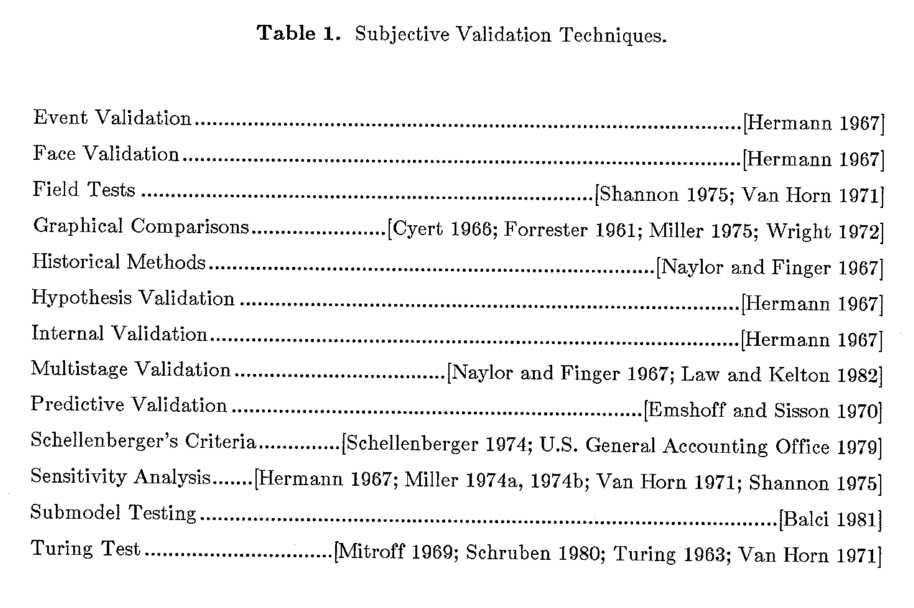
\includegraphics[width=.9\linewidth]{subjective_balci.png}
  \end{sidecaption}
\end{figure}

Ces deux citations permettent de montrer au passage comment la vision de la validation défendue par Hermann a été intégrée dans une forme très approchante par des acteurs de la \textit{V\&V} comme Balci ou Sargent, dont on a vu précédemment les définitions dans la section \ref{ssec:def_generique_validation}. Ces deux derniers sont en réalité les acteurs majeurs d'une synthèse (voir la figure \ref{fig:S_syntheseBalci}) opérée dans les années 1980-1990 \autocite{Nance2002}, dont on peut dire qu'elle est marquée par un retour à une certaine forme de neutralité (voir par exemple le rejet des aspects philosophiques décrits décrits dans la section \ref{ssec:def_generique_ validation}  qui se double d'un jargon technique spécifique à l'établissement d'un processus qualité exploitable pour l'ingénierie) . Des adaptations qui permettent probablement de mieux accepter en son sein des typologies de techniques aussi différentes que celle de Naylor\Anote{naylor_etonnement} ou Hermann. Régulièrement révisées, \textcite{Balci1998} fait ainsi état dans sa dernière taxonomie d'un catalogue de 75 techniques différentes dans lequel peuvent piocher les modélisateurs en fonction de leurs besoins. 

On se rend bien compte que dans le cadre des sciences humaines et sociales la possibilité de fixer par avance ce type de seuil n'a pas de sens, surtout dans un cadre explicatif.

%\textit{Que faut il entendre ici par partiellement ? Quels sont les leviers permettant au géographe de compenser cette perte de représentativité par un gain en compréhension sur le système à étudier ? }

Pour mieux comprendre quel est l'enjeu de cette délimitation entre un modèle réaliste et un modèle abstrait il faut évoquer cette tension permanente qui nourrit les choix du modélisateurs dans la construction d'un modèle explicatif. Deux attracteurs possibles et apparemment opposés, avec d'une part la volonté de se rattacher à une forme de réalisme au travers de l'injection d'une part maitrisée de réalité tout au long du processus de construction \Anote{durand_observation}, et d'autre part une force qui nous pousse au contraire à se détacher de cette même empirie pour ne retenir que le matériel susceptible de servir l'objectif du modèle.

La sociologue et épistémologue \textcite{Bulle2005} a bien formalisé ce dilemme dans la nécessité pour tout modélisateur de positionner son modèle sur un gradient opposant le réalisme des causes des modèles explicatifs \Anote{bulle_modele_explicatif}, au réalisme des effets des modèles descriptifs. 

Pour mieux comprendre quelles connaissances peut-on attendre d'un tel positionnement sur ce gradient, le mieux est encore de commencer par évoquer un de ses extrêmes, en invoquant par exemple le modèle universellement connu de Schelling. De par sa portée d'application extrêmement générale et la nature très abstraite de ses paramètres celui-ci constitue en soi un extrême intéressant pour comprendre où se situe encore l'explication lorsque le détachement de la réalité est à ce point éloigné. Sur ce point, les analyses de \textcite{Bulle2005} et \textcite{Phan2008, Phan2010} se réfèrent principalement à l'essai de \textcite{Sugden2002} pour évoquer quels types de relations entre les deux mondes peut on attendre de ce type de modèle épuré. 

Les résultats qui dérivent de la mise en dynamique des règles dans le modèle de Schelling sont d'une telle universalité, d'une telle robustesse qu'il n'est plus question de confronter les résultats ainsi obtenus à la réalité. A cet égard le potentiel explicatif de ce type de modèle s'oppose selon \textcite{Bulle2005} à tout réalisme empirique. De ce point de vue, \enquote{le modèle n'est pas tant une abstraction de la réalité qu’une réalité parallèle [...] bien que le monde du modèle soit plus simple que le monde réel, celui-ci n'est pas une simplification de l'autre. Le modèle est réaliste dans le même sens qu'un roman peut être appelé réaliste [...] les personnages et les lieux sont imaginaires, mais l'auteur doit nous convaincre qu'ils sont crédibles } \autocites[131]{Sugden2002}[10]{Phan2008}

L'effet d'une telle recombinaison d'hypothèses revient à mettre en oeuvre un \enquote{monde crédible} où l'inférence inductive est mobilisée pour identifier des similitudes significatives entre les deux mondes. \autocites{Livet2006, Phan2008}. Tout le travail réside donc dans l'interprétation prudente qui peut être faite entre ces résultats d'un monde factice et d'une réalité.

Un processus commun utilisé dans toute oeuvre de fiction pour piquer la curiosité de l'observateur, la mise en exergue volontaire d'une tendance du monde réel dans un monde imaginaire permettant d'entamer une réflexion sur l'existence, la portée, la nature de cette même tendance dans le monde réel. Les villes ou les sociétés mis en avant dans des oeuvres de fiction cinéma ou dans la littérature ne sont jamais que des mondes plus ou moins crédibles (Gotham City, 1984, Matrix, la série Black Mirror, etc. car la liste est longue ...)  pour mettre en avant un discours, ou des tendances du monde réel sur lequel doit porter le questionnement; (http://www.influxpress.com/imaginary-cities/ , \href{http://cybergeo.revues.org/1170#tocto1n9?}{cybergeo})

Si le discours scientifique n'a clairement pas cette obligation ludique, il n'en reste pas moins que ce processus de reconstruction crédible est déjà un outil formidable pour questionner les processus à l'oeuvre dans le monde réel \Anote{ruffat_samuel_ville}. Mais cette ambiguïté de lecture a déjà mené à de nombreux malentendus, d'une part envers le grand public (Voir forrester, mais également \Anote{deffuant_debat}) qui pourrait prendre des résultats de simulation pour la réalité avec tout les conséquences que cela suppose, mais également parfois entre scientifiques provenant de divers horizons. Ainsi après la lecture de la critique par \textcite{Chattoe2011} de l'article de \textcite{Yanoff2009}, il ressort toute la difficulté d'évaluer la méthodologie et le travail réalisé autour d'un modèle au travers d'une seule publication, notamment lorsque la fonction cognitive recherchée par les modélisateurs n'est pas décrite explicitement, ce qui provoque aussi ce décalage entre attente du lecteur et le processus réel de recherche qui sous-tend la construction du modèle. \hl{dp: TROP ALLUSIF}

\textit{Doit on se contenter de ce seul mode explicatif ? Existe t il un moyen pour renforcer la confiance dans la capacité explicative des hypothèses ainsi mobilisés ? } 

\paragraph{Justifier des hypothèses par leurs qualités de représentations}
\label{justifier_hypothese}

%% DEBUT - EN ATTENTE DE LA REPONSE DE VARENNE %%
\textcite{Bulle2005} evoque bien l'existence de modèle à cheval entre potentialité explicative et potentialité descriptive. Ainsi \enquote{appliquée aux processus sociaux réels, la simulation peut allier au potentiel descriptif offert par l’imitation d’effets empiriquement observables, le potentiel explicatif que lui confère la mise en œuvre de relations causales effectives. }

A la différence de modèles trop simples qui n'offrent que de maigres accroches avec la réalité, c'est donc par la réintroduction maitrisée de l'empirie dans les modèles de simulation construits que l'on pourrait espérer la mise en route progressive d'un processus de Validation ?

Un tel processus de justification parait complexe, car celui-ci ne peut être concu de façon homogène sans se heurter avec l'objectif même de toute modélisation, qui on le rapelle, n'est pas une construction guidée par la Validation mais une reconstruction mettant en oeuvre une simplification orienté par et pour un but. On ne parle pas d'un modèle comme d'un ensemble d'hypothèses de représentation homogène mais d'un ensemble d'hypothèse aux représentation hétérogènes.

Ce terme de \enquote{simplification} souvent employé reste d'emploi ambigue, la modélisation nécessitant comme le dit \textcite{Haggett1965} non pas tant la mise en oeuvre d'une simplification aveugle, qu'une idéalisation guidé par la volonté de mettre à nu des propriétés du système observé. \textcite{Brunet2000}, pour qui la modélisation est également un processus de recherche, propose même pour éviter toute confusion sur les termes de dénuder la définition de modèle de cette fausse directivité, le modèle devenant dans sa version la plus épurée une \enquote{représentation formalisée d'un phénomène}; le terme \enquote{représentation} intégrant alors toute la complexité sous jacente à une telle formalisation : \enquote{Il va de soi que cette représentation passe par plusieurs filtres, qui tous tendent des pièges : la perception du phénomène, sa représentation, la construction d'un modèle, l'interprétation du sens de ce modèle et la capacité du modèle à rendre compte du phénomène.}

Un point de vue semble-t-il partagé par Franck Varenne pour qui le terme simplification est \blockquote[{\cite{Varenne2008}}]{[...] un glissement d’attribution indu. Puisque l’usage du modèle est relatif (à un observateur et à un questionnement), on ne peut dire que le modèle doit être un objet simple en lui-même ou dans l’absolu. Il convient donc de regarder sous quel aspect exactement il doit apparaître simplificateur, sous quel aspect il devient un outil facilitateur, un outil de facilitation. [...] on comprend déjà qu’un modèle n’est pas ce qui est recherché en tant que tel, mais ce qui facilite la recherche d’information au sujet d’un système réel ou fictif, cela dans le cadre d’un processus à visée de représentation, de connaissance, de conceptualisation, de conception ou encore de transformation. Il est le moyen plus que la fin. C’est pourquoi je m’aventurerai, à partir de maintenant, à user plutôt du terme de facilitation que de celui de simplification [...]}

Comme déjà évoqué par les géographes, ce n'est pas tant \enquote{le modèle} que ce qu'il y a \enquote{dans le modèle} qui nous intéresse \autocites{Sanders2000, Besse2000}.

Seulement comment analyser la pertinence d'une représentation prise en dehors de son contexte ? Les choix intervenant lors d'une modélisation ne répondent pas à une logique universelle pré-établie, et sont motivés et modulés par un ou plusieurs objectif(s) qui n’interviennent pas forcément de façon volontaire pour guider la modélisation. \textcite{Varenne2013} ayant par ailleurs identifié une vingtaine de ces \enquote{fonctions de facilité de médiation} pouvant très bien se cumuler lorsqu’on observe un modèle. Or il me semble qu'une fois rapporté à la structure interne du modèle de simulation, on est bien obligé de constater l'impact que peut avoir cette diversité d'objectifs dans la mobilisation d’une ou plusieurs représentations, dont certaines peuvent être concurrentes, pour une même hypothèse dans le modèle. Est-ce pour dénoter une entité réelle (un agent = un individu, une ville, une innovation ) ? Est ce dans le but de simplifier pour la compréhension ? pour les performances ? pour répondre au principe de parcimonie ? Ou tout à la fois ? (une population agents homogène devenant une équation de croissance par exemple ) Était-ce un choix fait à la suite d’une multitudes d'autre essais (différentes équations plus ou moins représentative du phénomène à considérer) ? etc. Dans le cas d'un modèle de migration inter-ville, il est en effet plus intéressant de mobiliser les populations de façon agrégé si on s'intéresse aux règles intervenant dans la dynamique d'interactions entre les villes, par contre, si il s'agit d'observer l'impact que peuvent avoir des règles de comportements sur ces interactions, ce niveau peut devenir pertinent; cette approche ne chassant évidemment pas la première, au contraire les couplages étant bienvenu. En définitive, il n'y a aucune raison pour que les hypothèses intégrées aux modèles de simulation soit homogènes. Ainsi, pour Franck Varenne, pour identifier à posteriori quels sont les fonctions épistémiques mobilisés, et donc par extension déterminer dans quelle mesure l'intérêt porté à la validation a pu être très diffèrent lors de la construction du modèle (pour un modèle de simulation pédagogique, la validation n’est par exemple clairement pas une priorité ...), il est nécessaire de se poser la question pour chacune des hypothèses représentées dans le modèle de simulation : est ce une dénotation ? une exemplification (métaphores) ?

Normalement tout ces choix devrait être explicités \autocite{Varenne2013b}, ce qui est rarement le cas, vu la complexité d'une tâche qui apelle pour être sérieuse l'analyse d'une activité de raisonement accompagnant le modèle dont les jalons ont bien souvent disparu.

La tendance à la pluriformalisation \Anote{pluriformaliser } permise par les modèles multi-agent ne vient pas non plus faciliter cette tâche, car ces modèles de simulation qui peuvent déjà intégrer -et c'est d'ailleur pour cela qu'ils ont autant de succès- sans problème une hétérogénéité d'échelle, de niveau d'abstraction, de modèles, doivent aussi compter avec l'intégration de formalismes mobilisant des temporalités et/ou des échelles différentes \autocites{Varenne2008,Varenne2012a}. Ces couplages n'étant pas toujours évident, y compris au niveau informatique où des artefacts (c'est à dire l'apparition de mécanismes nécessaire à l'implémentation mais non prévu et difficile à expliquer d'un point de vue purement théorique) peuvent venir rapidement venir perturber les ontologies réalisés en amont. 

Même les modélisateurs ont parfois du mal à s'y retrouver, par exemple il n'est pas toujours évident d'expliquer pourquoi on a choisit de coupler pour certain mécanismes le formalisme agents avec celui des équation différentielle ? Il faut alors comprendre que dans certains cas, c'est aussi ce qui a pu motiver le modèle, l'intérêt de la pluriformalisation étant justement ce qu'il faut démontrer en comparaisons des approches traditionnelles prisent séparément. Plusieurs réflexions ont montrés qu'il s'agissait d'un type de modélisation en devenir et en voie de démocratisation, les formalismes pour la simulation informatiques (multi-agents, micro-simulation, automates cellulaires) ou mathématiques (systèmes dynamiques) utilisés n'ayant jamais eu vocation à s'opposer (approche individu - centré contre approche mathématique traditionnelle) comme on aimerait parfois nous le faire croire \autocites{Sanders2013, Banos2013}. 

\textcite{Varenne2013b} s’intéresse de beaucoup plus près aux effets de cette hétérogénéité interne aux simulations d’un point de vue épistémologique, et c’est d'ailleurs de ces articles sur cette question et de plusieurs échanges privés avec lui qui ont inspirés certaines de ces dernières réflexions. Il nous sera toutefois difficile d’aller au delà sur cette analyse de la \enquote{représentativité des hypothèses fonction des objectifs}, car même si celle-ci est une question passionnante, elle reste un axe de recherche avant tout théorique et en plein développement. Aucun n'exemple concret ne permet pour le moment d'illustrer la forme que pourrait prendre une telle analyse.

Un autre argument vient condamner encore plus fermement l'idée de justifier d'une Validation des modèles basée sur la qualité de représentation de ses hypothèses. Celui-ci a déjà été effleuré en traitant de philosophie des sciences dans la section \ref{sssec:philo_sciences}. Le processus de validation se heurte rapidement à la différence de nature entre les résultats produits par des hypothèses \textit{reconstruites} et le monde réel \Anote{bulle_modele_autonome}. Tout comme le substrat est artificiel, le résultat produit par cette dynamique reste le produit d'un monde reconstruit - \textit{in silico} - L'existence de ce nouveau niveau d'empirie amène les épistémologues comme Franck Varenne à parler ici d'\enquote{expérience concretes du second genre} faisant alors de la simulation une \enquote{quasi-expérimentation} \autocites{Varenne2001, Varenne2007, Phan2008}

On en déduit que quelque soit notre placement sur ce gradient, il est effectivement vain de chercher à valider un modèle en usant d'un quelconque \enquote{seuil de suffisance} caractérisant \enquote{l'injection de réalisme à atteindre qui autoriserait une inférence certaine sur le monde réel}, puisque de toute façon cette inférence s'appuie sur un résultat \enquote{artificiel} forcément discutable \Anote{phan_livet_modele}.

\paragraph{Inverser le problème de la validation pour désengager cet objectif de correspondance au réel}
\label{p:inverser_problematique}

Une autre façon donc de dépasser cette problématique de la Validation est d'accepter le fait que le réalisme des hypothèses ne soit plus vraiment un objectif, mais plutôt la réalisation conséquente d'une expertise qui tient essentiellement de l'angle théorique choisi pour éclairer un problème.

Autrement dit, la confiance établie dans les capacités explicatives des hypothèses choisies ne se juge pas tant dans la comparaison des résultats attendus avec le réel observé, que dans l'exploration du monde crédible ainsi simulé en fonction de critères experts construit sur une observation du réel, dans l'espoir d'en dégager une connaissance qui doit encore être vérifiée \Anote{denise_geopoint}. 

Le problème est ici en quelque sorte inversé, ce n'est plus une qualification directe du réel qui est visé par le modèle, mais le modèle qui est visée par notre compréhension du réel au travers de critères experts. Ceux-ci viennent questionner et mettre en tension ce monde virtuel en lui imposant de nouvelles contraintes, révélant par là même les forces et les faiblesses de nos hypothèses dans le modèle. On oppose dans la construction du modèle \enquote{un jeu d'hypothèses susceptible de produire des résultats attendus}, à la réalité des conclusions apportés par la \enquote{mise en oeuvre effective d'une dynamique}.

Cette situation semble ramener le problème de la \enquote{Validation} à une évaluation \enquote{terme à terme} entre hypothèses et critères devant en rendre compte. 

C’est me semble-t-il ce que voulais dire Frédéric Amblard \textcite{Amblard2006} lorsqu’il parle du rapport liant la détection de comportements de la \enquote{validation interne} à leur utilisation comme support d’une partie de la \enquote{validation externe}.  

\blockquote[\cite{Amblard2006}]{L'analyse de sensibilité, si elle peut s'appliquer pour tester la robustesse des résultats d'un modèle, peut également être utilisée pour tester la robustesse de la structure du modèle. En modifiant les hypothèses réalisées dans le modèle, par exemple en modifiant les structures organisationnelles, le modélisateur obtient des indices relatifs à la stabilité de son modèle et de ses hypothèses. Ces indices lui permettent précisément de jauger l'importance du choix d’une hypothèse et l’influence de son remplacement par une autre sur un aspect particulier du modèle. [...] Une autre propriété importante qu'il s'agit d'étudier au cours de cette étape de validation interne, concerne les classes de comportements produites par le modèle. Les simulations multi-agents produisent ce qui est assez communément appelé des \enquote{comportements émergents }  (voir chapitres 14, 16 et 17), c'est-à-dire des comportements qui ne sont pas exprimables en utilisant uniquement les hypothèses réalisées sur les comportements individuels}.

Deux propriétés qui font ainsi écho à une méthode de la validation externe qui \enquote{[...] consiste à rapprocher les classes de comportements (identifiées lors de la validation interne) à des comportements saillants du système-cible : les faits stylisés.}


\enquote{Ce rapprochement, s’il peut être fait avec des faits stylisés identifiés a posteriori (permettant par exemple de découvrir dans les phénomènes empiriques, des comportements stylisés qui auraient pu passer inaperçus), possède, on le sent bien, plus de force lorsque les faits stylisés sont déterminés avant même la modélisation comme des comportements que l'on cherche à reproduire par le modèle ou dont on se servira comme un critère de validation parmi d'autres (rétrodiction).}\autocite{Amblard2006}

% A CORRIGER
Ce points nous incite également à pratiquer une évaluation à contrepied de la démarche habituelle, alternant validation interne, puis externe. Le modélisateur se saisit un moment de cette légitimité évoqué par \hl{Bulle} en devenant celui qui met en tension cette relation pour construire ses modèles. On met alors de coté un instant la validation interne comme exploration non dirigé des comportements du modèle pour se concentrer sur une exploration, moins complète, ou c'est ce désir de rapprochement qui vient piloter cette fois ci l'exploration des comportements. Les modélisateurs peuvent en effet introduire les hypothèses dans un modèle de simulation dans le but de satisfaire, ou \textbf{de ne pas satisfaire} ces critères. 

En effet on a bien précisé par exemple que l'objectif de correspondance avec les données n'était plus un critère prioritaire dans l'établissement de tels modèles de compréhension, sinon pourquoi ne pas se contenter d'un simple modèle de Gibrat pour expliquer la hierarchisation des systèmes de villes ? 


%Cette inversion soulève de nombreuses remarques que l'on va tenter d'articuler par la suite. 
Cette inversion soulève plusieurs remarques. D'une part, on se rend compte que les critères d'évaluation deviennent aussi importants que les hypothèses dont ils sont censés rendre compte. D'autre part, il faut soulever les modalités qui sous tendent cette nouvelle façon de construire de la connaissance. C'est par ce dernier point que nous allons commencer notre analyse.

\paragraph{L'abduction, un phénomène clef moteur dans l'activité de modélisation}
\label{p:abduction}


La présence d'une hypothèse dans le modèle se justifie donc autant par l'expertise du modélisateur que par son adéquation, ou sa non-adéquation \textbf{potentielle} avec différents critères de validation. La subjectivité de l'expérimentateur joue sur les deux tableaux, et donne à voir dans cette subtile inter-dépendance qui relie le choix des hypothèses et le choix des critères une forme d'incertitude quant au résultat assez difficile à prévoir et quantifier.

Que se passe-t-il en effet lorsque le potentiel explicatif d'une hypothèse pourtant appuyé par des résultats empiriques constatés dans le système observé s'avère invalidée par une analyse de sensibilité ou un critère d'évaluation ? Et cela, alors même que l'experimentateur considère celle-ci comme étant indispensable au développement d'une dynamique donnée ? Que se passe-t-il au contraire lorsqu'un critère d'évaluation est atteint alors que cela n'était pas attendu au vu de la structure actuelle du modèle ? 

%La fonction heuristique de la simulation pouvant s'exprimer tout autant dans cette \enquote{surprise} d'une divergence entre le potentiel investit dans les hypothèses et les critères selectionnés, que dans la surprise suivant l'introduction de nouveaux critères contraignant le modèle, et remettant en cause ce même potentiel de représentation investit dans certaines hypothèses. 

Il y a une divergence nécessaire entre la volonté du modélisateur de rendre compte d'un système observé par un réseau d'hypothèses qui lui paraît parcimonieux, nécessaire et cohérent d'un point de vue thématique (le potentiel investi), et la réponse effective apportée par la mise en dynamique de ces causalités lues au travers des critères selectionnés pour en rendre compte. % la possibilité d'infirmer ou d'affirmer de nouvelle connaissances, avec le développement de nouveaux critères, de nouvelles hypothèses ayant jusque là échappé aux raisonnement du modélisateur.

\foreignblockquote{english}[{\cite[219]{Hermann1967}}]{In developing a game or simulation, the designer is required to be explicit about the nature and relationships between the units in the operating system and their counterparts in the observable universe. He must specify the conditions which cause a relationship to vary. In constructing an operating model a connection between previously unrelated findings may be discovered. Alternatively, a specific gap in knowledge my be pinpointed and hypotheses required by the model my be advanced to provide an explanation.} 

La surprise volontaire ou involontairement produite au cours de cette divergence, et qui accompagne généralement l'activité de modélisation, revient sous le nom d'abduction, le terme venant de Charles S. Peirce \autocites{Besse2000, Banos2013, Phan2006, Livet2014} 

On a déjà précisé en s'appuyant sur les propos de Ian Hacking \autocites{Hacking1989,Hacking2003, Hacking2006} que ce phénomène d'abduction n'était pas un héritage du seul cadre logique, mais une propriété inhérente à l'humain \Anote{stanislas}, existante de façon préalable à ses créateurs Aristote, ou Peirce. 
%Cette logique bayésienne qui consiste à formuler une hypothèse a priori de façon consciente ou inconsciente \Anote{kauffman}, prise de façon rapide ou lente, basé sur nos connaissances passés ou sur notre environnement présent, pour la confronter et la réévaluer au yeux de la réalité de façon itérative correspond assez bien il me semble à ce que l'on pourrait apeller \enquote{abduction}, apellée également \enquote{inférence de la meilleure explication}. 

Dans l'utilisation des modèles de simulation d'une part ce n'est pas le monde réel qui nous surprend, mais ce qui se passe dans le modèle de simulation, et d'autre part il est plus intéressant d'adopter une démarche active et créative dans la mobilisation des hypothèses, afin de maximiser la surprise plutôt que de la miminiser, de dépasser son horizon de connaissance plutot que de s'y conforter. Comme le résume bien \textcite{Banos2013} dans son HDR, \enquote{l’esprit même de l’abduction au sens de Peirce, désignant cette capacité de l’être humain à générer des hypothèses temporaires à partir de l’information incomplète dont il dispose. Appliquée à la démarche scientifique, l’abduction renvoie ainsi à la capacité du scientifique à se mettre en position d’étonnement, à se laisser guider par la recherche de l’inattendu et plus généralement à laisser libre cours à sa créativité.} 

Comme on pouvait alors s'y attendre, les motifs développés par les modélisateurs soutenant cette approche sont très loin de ceux attendus pour la prédiction, ou c'est d'abord la robustesse des résultats qui prime, car \enquote{[...] dans le cas d’une modélisation compréhensive, où l’objectif est d’apprendre des propriétés du système que l’on reconstruit \textit{in silico}, le fait d’avoir, pour une partie des conditions expérimentales des comportements très erratiques du système, loin de discréditer le modèle nous apprend au contraire des éléments de son fonctionnement et nous permet même d’anticiper le fonctionnement du phénomène modélisé. Si sous certaines conditions le modèle est très instable c’est une information très enrichissante sur le modèle et sur le phénomène considéré.} \autocite{Amblard2010} 

Force aussi de constater que cette incrémentalité dans la construction d'un modèle de simulation ne suit pas vraiment un modèle linéaire de développement, et s'accompagne, au moins dans les sciences humaines et sociales d'une activité de raisonnement en partie imprévisible. Ainsi il peut paraître paradoxal pour un modélisateur débutant de voir à quel point il est important de \enquote{malmener} les modèles que l'on a précédemment construits avec raison et parcimonie. L'important ici nous dit \textcite{Amblard2010}, c'est que cela participe à l'élaboration de la compréhension ou de l'explication des phénomènes considérés. Car comme le dit \textcite[65]{Banos2013} dans son tout premier principe, modéliser c'est avant tout apprendre.

D'autre définitions de l'abduction \Anote{abduction_definitions} permettent de mettre en valeur d'autres de ces propriétés, la création en est une, mais avec celle-ci vient aussi la sélection. Si on se rapporte aux processus de cognition, la conscience apparaitrait par exemple comme un filtre discrétisant, sélectif, d'une pensée inconsciente fluctuante et résolument continue. On peux supposer que lors de la modélisation, ce type de processus est également à l'oeuvre, et il n'est pas rare lorsqu'on construit un modèle de simulation d'avoir à choisir, ou à ne pas choisir, avec plusieurs hypothèses ou implémentation d'hypothèses alternatives. Le deuxième choix expliquant aussi en partie pourquoi les interfaces utilisateurs de nombreux modèles de simulation Netlogo sont aussi riches en boutons de sélection...


%Cela soulève la possibilité d'hypothèse explicative concurrente ou inter-dépendante dans l'apparition d'un phénomène, dont certaine échappe forcément au seul modélisateur géographe du fait par exemple de la nature inter-disciplinaire des objets engagés, auquel il faut encore appliquer une selection plus consciente en décidant de mettre plus ou moins en avant des hypothèses susceptible de surprise. 

%La surprise ne vient donc pas seulement du modèle, mais aussi de ce que font les autres manipulant les modèles, surtout dans le contexte inter-disciplinaire ou nous évoluons, les limites de nos connaissances se manifestant assez vite lorsqu'il s'agit d'étudier un phénomène ou un objet partagé, comme les villes par exemple. 


\paragraph{Quels critères d'évaluation pour quelle mesure des hypothèses ?}
\label{p:critere_evaluation}


% S'exprime dans une dynamique ? 


Il y a plusieurs problèmes qui limitent cette possibilité d'une comparaison directe avec les données. Au tout début de notre argumentaire, on a vu avec Hermann que la mobilisation d'un seul critère quantitatif ne pouvait pas suffire à garantir une quelconque explication. Avec suffisament de degré de liberté, que cela soit par le nombre d'hypothèses mobilisés, ou le nombre de paramètres que l'on met à disposition d'un optimiseur humain ou ordinateur, on trouvera toujours un moyen de correspondance aux données. Amblard parle de surdétermination des paramètres aux données \hl{vérifier ici.}.

%Problème de nature des données, et de leur disponibilités
Un autre problème se pose également avec la mobilisation des données. Du fait de l'\textit{Observational Dilemna}, cette solution d'une comparaison terme à terme explicite entre hypothèses constituantes du modèle et critères n'apparait pas faisable selon \textcite{Batty2001} : \foreignquote{english}{In principle, each element of this process should be explicit and should be capable of being validated with observed data. In practice, this is rarely if ever the case. The data set would be too large, it would be impossible to collect in its entirety, it may be impossible to even observe and measure. Yet the processes are known to be important. Other criteria must thus be used.} 

On peut ajouter à çà une autre limite concernant les données, on a effet vu que toutes les hypothèses du modèles n'avaient aucune raison de se placer au même niveau d'abstraction, ou d'appartenir au même formalisme. Il est par exemple déjà difficile d'accéder à des données dans une fenêtre spatio-temporelle donné, est-il possible d'en avoir sur plusieurs fenetres, voire plusieurs fenetres simultanées ? 

Le dilemne commence à apparaitre clairement, car il ne s'agit pas de tomber dans une \foreignquote{english}{Forrester Strategy}, en abandonnant toute volonté de justifier la chaine d'hypothèses mobilisés dans les modèles.

% multiplication des critères ?
On peut de nouveau faire appel à l'analyse d'Hermann, dont l'originalité réside aussi dans les remarques très juste et très précoce qu'il a formulé sur la relativité des hypothèses \textbf{mais aussi des critères mobilisés} dans les modèles. Celui-ci est en effet tout à fait conscient qu'il ne s'agit pour l'une comme pour l'autre que d'assertions sur la réalité. Il propose donc d'essayer de faire au mieux. En adoptant une validation multi-critère \Anote{methode_hermann} intégrant les objectifs ayant guidé la construction du modèle, il espère ainsi renforcer le crédit qu'il est possible d'apporter aux simulations, et reste sceptique sur la possibilité d'inférer en retour sur les systèmes observés.

\foreignblockquote{english}[\cite{Herman1967}]{We have arrived at the position, then, that multiple validity criteria are needed because of the error of measurement and because of the recognition that criteria can be only assertions about \enquote{reality}}

Pour \textcite{Amblard2006}, si cette validation externe basé sur une comparaison quantitative avec les données n'est pas impossible, elle n'en reste pas moins difficile à mettre en oeuvre de façon systématique, en partie pour les raisons évoqué ci-dessus. L'appel à des critères d'évaluation plus qualitatif (\enquote{fait stylisé}) reste le plus évident à mettre en oeuvre. Un point de vue partagé par \textcite{Batty2001} \foreignquote{english}{ [...] complex systems models have multiple causes which display a heterogeneity of processes that are impossible to observe in their entirety. The focus is on more qualitative evaluation of a model’s plausibility in ways that relate to prior analysis of the model’s structure.} 

Cette démultiplication des critères d'évaluation, même si c'est une opération qui reste indispensable, ne nous sauvera pas d'un autre problème. Il n'y a pas de seuil de suffisance à chercher dans la représentativité des hypothèses, mais également dans leur mise en cohérence/relation, puisque celle ci comme les deux autres tient d'une reconstruction guidé par une but. La recherche d'une cohérence interne au modèle n'apporte pas plus de garantie sur la transférabilité des hypothèses à la réalité. Ce qui ne veut pas dire qu'il ne doit pas y'en avoir, seulement celle-ci doivent être faite pour les bonnes raisons, et non pas pour se donner l'illusion d'une meilleure inférence des conclusions du modèle au système observé.

\foreignblockquote{english}[\cite{Osullivan2004}]{There is a many to one relationship between the structure of models and the behaviour they produce, so that many models can account for the same observed outcome. This is the equifinality problem. One common (incorrect) response to the problem is to examine the internal consistency of the model, and to assume that internal consistency guarantees a true representation of reality. Alternatively, we resort to calibration, and adjust model parameters until a best fit to historical data is achieved. Calibration is a complex technical procedure, but ultimately offers no escape. At best, observational data can be replicated more or less closely, but this provides no guarantee as to a model’s accuracy as a representation, nor does it exclude any other model, or another choice of parameters.}

Outre donc la question de la disponibilités des données en sciences humaines et sociales, l'\textit{Observational Dilemna} sous-tend également l'impossibilité d'établir l'unicité des hypothèses avancées pour décrire un phénomène, mais aussi par extension celle des critères d'évaluation, qui reste eux aussi des construits formulés sur la base d'une observation du système observé. Capturer toute la substance d'un phénomène émergent dans un ou plusieurs critère d'évaluation reste difficile, voire impossible.

Cette variabilité exprimé dans la construction et la paramétrisation des structures causales et des critères associés renvoie à ce phénomène bien connu des modélisateurs en sciences humaines et sociales, à savoir l'équifinalité.

L'équifinalité est un terme provenant à l'origine d'un phénomène observé en embryologie \Anote{embryon}, généralisé ensuite par Bertalanffy comme \textbf{une propriété fondamentale des systèmes ouverts} (voir la section \ref{subsec:gst} en annexe pour une remise en contexte du terme). Celui-ci reste un terme couramment employé dans la littérature, et que l'on retrouve associé à une limitation dans la \enquote{Vérification} (à ne pas confondre avec la Vérification de la Validation \& Verification ... \autocite{David2009})  en philosophie : \foreignquote{english}{\textcite{Oreske1994} crisply describe the problem: it is impossible to verify the representational truth of any model of an open system. There is a many to one relationship between the structure of models and the behaviour they produce, so that many models can account for the same observed outcome. This is the equifinality problem.} \autocite{OSullivan2004}

Pour \textcite{Bulle2005} il sera donc toujours nécessaire et légitime de questionner la pertinence des rapports mesurés entre les liens causaux proposés dans le modèle et le ou les critères qui sont censés en rendre compte.

\hl{T:} 
Cette variabilité est à la fois conséquence naturelle du processus de raisonnement, mais également une conséquence logique liés à la nature insaisissable du réel. Toutefois là ou on pourrait voir cet effet comme positif et cumulatif, l'équifinalité est souvent présenté comme un défaut de l'outil et de la discipline. La section suivante essaye de voir les solutions proposés par la communautés des modélisateurs dans la mise en perspective d'un débat récent. Une autre proposition, plus proche de nos pratiques sera ensuite présenté, mais nécessitera de repenser la façon dont sont construit et valorisé des modèles. % dans un cadre d'analyse qui s'appuie sur l'existant pour mettre en valeur les aspects dynamique, cumulatif, et local de cette activité.

\subsubsection{Repenser la question de l'équifinalité}

On a vu dès le départ avec Hermann que la validation était indissociable d'un contexte, et posé de fait la question de la représentativité des hypothèses à celle des critères mobilisés. 

En cherchant comment pouvait-on mesurer de la qualité explicative des modèles réalisés, on s'est apercu que la recherche d'un seuil de réalisme adéquat n'était pas un bon argument pour guider l'intégration des hypothèses sur les entités ou les activités à injecter dans nos modèles.% En développant jusqu'au bout l'argument d'une justification possible dans le choix fait des modélisateurs sur la représentativité des hypothèses, on s'est rendu compte qu'il s'agissait pour le moment plus d'une question épistémologique a posteriori que d'un comportement assumé par les modélisateurs. Peu de modélisateur font aujourd'hui cet effort d'explicitation des fonctions facilitantes associés à chacune des hypothèses en les rapportant au raisonnement accompagnant la construction du modèle.

Enfin, comme il n'est pas non plus possible de garantir une validation empirique terme à terme entre hypothèses et données, il est nécessaire d'accumuler différents critères quantitatifs et qualitatifs non pas pour se rapprocher d'un fonctionnement réel, mais plutot là aussi pour garantir la cohérence d'une \enquote{reconstruction d'un jeu de causalité identifié dans l'observation d'un phénomène} que l'on veut confronter \enquote{aux mesures censés rendre compte de ce phénomène dans la réalité}. Le jeu abductif entre en compte pour encourager ou perturber ce rapprochement entre hypothèses selectionnés et critères mobilisés.

Il a été avancé également qu'une partie des connaissances dégagés durant ce jeu abductif rythmant la construction des modèles était lié au fait que le modèle de simulation servait de laboratoire non pas pour modéliser et confronter le monde réel, mais plutôt pour modéliser et confronter nos a priori théorique sur le fonctionnement du monde observé. A ce titre, les échecs induisent un retour sur la théorie plus stimulant que les réussites, ce qui motive aussi la prise de risque et la créativité dans les hypothèses ou les critères avancés.

Chacun de ces arguments renvoie normalement l'image d'une activité de validation indissociable d'un contexte donné. Pour reprendre les mots de \textcite{Amblard2006} \enquote{[...] les questions pour la validation des modèles ne devraient jamais être abordées en dehors des questions relatives à leurs usages.} 

L'équifinalité vient ici compliquer ce constat, car elle fournit l'image inverse si on n'y prend gare, en facilitant l'idée qu'une construction peut être facilement remplacé par une autre, sans que le contexte ne soit abordé. Le problème n'est pas que cela puisse être vrai ou faux, car comme on va le voir ensuite, la possibilité de rendre compte différemments d'un même phénomène a été intégré depuis longtemps dans les différentes modélisations supportées en géographie, mais plutot que des personnes extérieures à une communautée puissent penser que c'est un défaut des techniques ou des méthodologies utilisés, alors que c'est un défaut propre à l'études des systèmes complexes, et donc également des systèmes sociaux. 

Une entrée par les critiques récentes formulés sur ce cadre d'analyse historique des \enquote{Science Générative} formulé par Epstein peut être un bon exemple pour montrer que l'équifinalité, si on ne la justifie pas, peut grever la crédibilité des modèles présentés. Elle peux même comme on va le décrire dans la section suivante, fournir le support biaisé à un argumentaire qui décrédibilise l'apport explicatif permi par l'utilisation de cet outil en en sciences humaines et sociales. Un groupe de sociologues proposent de répondre à ces critiques par un nouveau cadre d'analyse. 

%Débat CONTE / EPSTEIN, résoudre equifinalite en justifiant d'une causalite
\paragraph{Faire appel à un nouveau cadre d'analyse ?}
\label{p:cadre_analyse}


%L'etude de cette problématique de l'équifinalité à l'orée des débats ayant lieu dans une communauté inter-disciplinaire telle que celle gravitant autour du journal JASSS est intéressante car elle introduit chez les sociologues un cadre pour penser la construction et l'évaluation des modèles, d'origines assez ancienne, qui intègre certains des éléments discutés précédemment : \enquote{les mécanismes générateurs}.

C'est la faille emprunté par \textcite{Yanoff2008} qui s'appuie sur le modèle des Anasazi \autocites{Dean2000, Epstein2002} pour proposer une critique générale des \textit{Artificial Societies} \Anote{desuet_as}.

\hl{2 mots sur les anasazi, cf Clara ou Elsenbroich}

Ce modèle et sa dynamique ont été tant de fois fois répliqués, analysés et cartographiés que les défauts sont bien connu des modélisateurs. Malgré cela, ce modèle possède toujours une aura et une symbolique très forte, car il a ouvert la voie à d'autres modèles de simulation en archéologie, et en sciences sociales \autocites{Janssen2009, Stonedahl2010, Schmitt2013}[151]{Schmitt2014}. Le \enquote{motto} bien connu d'Epstein pour une \textit{generative social science} \foreignquote{english}{If you didn't grow it, you didn't explain its emergence} \autocites{Epstein1996} reste aussi une source d'inspiration pour de très nombreux modélisateurs, malgré les critiques. Grunne-Yanof n'ignore probablement pas donc que lorsqu'il s'attaque à ce modèle assez symbolique, il s'attaque aux pratiques de toutes une communauté dont il ne fait \textit{a priori} pas parti. 

Comme le résume bien \textcite{Elsenbroich2012} \foreignblockquote{english}[\cite{Elsenbroich2012}]{Grüne-Yanoff argues that this simulation does not give a causal explanation of the population dynamics of the Anazasi. The argument is not that the simulation is not an explanation of the Anazasi population but that it is not a causal explanation. The simulation does not tell a full causal history of the population dynamics, for example, the total exodus is not an outcome of any run of the simulation, thus leaving the explanation partial. Grüne-Yanoff argues that there is no such thing as a partial causal explanation. A causal explanation has to give a full account of all interactions leading to a phenomenon as there is no formal criterion to distinguish bad partial causal explanations from good partial causal explanations.}

Ce problème fondamental que tacle Grüne-Yanoff sans vraiment le nommer dans son texte, c'est l'équifinalité, et plus précisément l'équifinalité telle qu'ont peut la comprendre dans ce cadre d'analyse qu'est la science générative définis par Epstein.

Effectivement, même \textcite{Chattoe2011} qui critique de façon très virulente les propos de \textcite{Yanoff2008} doit bien admettre, avec d'autres, que l'existence d'un critère unique - qui plus est quantitatif - n'est effectivement pas suffisant pour juger de la qualité des hypothèses du modèle. Toutefois comme il précise ensuite, l'attaque mené par Grüne-Yanoff sur ce point envers les Anasazi reste une attaque elle aussi \textit{ad-hoc}, dont les conclusions ne peuvent en aucun cas être généralisé à l'ensemble des modèles de simulation en sciences humaines et sociales. Celui-ci ne faisant d'ailleurs dans sa démonstration aucun cas de l'existence d'une méthodologie sur lesquels les auteurs du modèle aurait pu se baser pour la construction du modèle \Anote{yanof_equi_a}, alors que celle-ci existe bel et bien dans les ouvrages de références. Une erreur que \textcite{Chattoe2011} juge difficilement pardonnable lorsqu'on s'adresse ainsi à toute une communauté, avec son histoire, ses méthodes, ses codes, ses discussions, ses ouvrages et articles de références. 

Il suffit d'ailleur d'évoquer cette question pour trouver dans \textcite{Epstein2006} une longue clarification de l'auteur au sujet de sa phrase si souvent reprise d'\textcite{Epstein1999} \textit{If you didn’t grow it, you didn’t explain it.}. Le constat qui en ressort est accablant pour Grüne-Yanoff : 

\foreignblockquote{english}[\cite{Epstein2006}]{The scientific enterprise is, first and foremost, \textbf{explanatory} [...] If you didn’t grow it, you didn’t explain it. It is important to note that we reject the converse claim. Merely to generate is not necessarily to explain (at least not well). A microspecification might generate a macroscopic regularity of interest in a patently absurd—and hence non-explanatory—way. For instance, it might be that Artificial Anasazi [Axtell, et al. (2002)] arrive in the observed (true Anasazi) settlement pattern stumbling around backward and blindfolded. But one would not adopt that picture of individual behavior as explanatory. In summary, \textbf{generative sufficiency is a necessary, but not sufficient condition for explanation.}} 

\textbf{La générativité n'a jamais été pour lui une condition suffisante à l'explication}, et l'équifinalité est un concept bien connu de l'auteur qui renvoie pour cet effort de selection entre les hypothèses la balle à chacune des disciplines. 

\foreignblockquote{english}[\cite{Epstein2006}]{Of course, in principle, there may be competing microspecifications with equal generative sufficiency, none of which can be ruled out so easily. The mapping from the set of microspecifications to the macroscopic explanandum might be many-to-one. In that case, further work is required to adjudicate among the competitors. [...] In any event, the first point is that the motto is a criterion for explanatory candidacy. There may be multiple candidates and, as in any other science, selection among them will involve further considerations.} 

Au regard de cette clarification, la formule de Macy est reprise parfois de façon un peu rapide comme ici : 

\foreignblockquote{english}[\cite{Marchionni2013}]{Thus, Macy and Flache (2009, 263) are right when they challenge J. M. Epstein’s slogan by claiming, \enquote{If you don’t know how you grew it, you didn’t explain it.} The idea of generation is necessary for explanatory understanding, but it is not sufficient.}

La levée de ce point montre bien à quelle point \textcite{Yanoff2008} avait oublié de préciser que la construction et l'évaluation d'hypothèses de comportement crédible était clairement l'intérét du modèle Anasazi, et non pas juste la réplication \enquote{aveugle} d'une régularité macroscopique par tout les moyens. Il n'a par exemple jamais été question de biaiser les hypothèses de ce modèle comme le laisse supposer \textcite{Yanoff2008} dans la comparaison que celui-ci fait avec le modèle de métérologie présenté par \textcite{Kuppers2005}, volontairement faussé pour prédire correctement. 

\textit{Que faut-il retenir d'une telle passe d'arme ?} Tant que les modèles publiés ne montre pas plus d'efforts pour décrire à la fois les démarches de modélisations ayant permis la construction des critères et des hypothèses, et l'activité d'évaluation qui autorisent leurs présences dans les modèles, le risque de voir ce type de publication se reproduire n'est pas écarté.

Parmis les autres critiques de \textcite{Yanoff2008}, on citera celle \textcite{Elsenbroich2012}. Comme \textcite{Chattoe2011} celle-ci insiste sur le fait que les problèmes avancés par Grüne-Yanoff ne sont en rien spécifique à la modélisation multi-agents, et se rapporte à l'ensemble des sciences sociales. C'est le cas par exemple la question de l'incertitude ou de l'absence des données mobilisés, l'équifinalité. Mais celle-ci revient surtout sur la partie explication avancé par ce dernier en lui donnant raison sur un point. Elle est d'accord pour dire que la simulation multi-agents, pas plus que les sciences sociales, ne peuvent effectivement ni fournir de chaine causale complète ou même d'explication potentielle \Anote{explication_potentielle}. Toutefois, et c'est là le plus important, \textcite{Elsenbroich2012} réfute la proposition de \textit{Functionnal Explanation} de Cummins proposé par Grüne-Yanoff. Nous n'avons pas la place de citer tout ses arguments, mais un seul devrait suffire à relever l'impossibilité d'adhérer à cette proposition (\textit{limit-problem}). En effet, pour \textcite{Elsenbroich2012} ce cadre explicatif ne permet tout simplement pas d'avancer des explications partielles : 

\foreignblockquote{english}[\cite{Elsenbroich2012}]{Grüne-Yanoff states that a full functional explanation is a causal explanation. This uniqueness is explicitly used in Cumins' Individuation criterion (below). The problem is that we will never have a causal explanation as we can never really be sure we have identified all the real entities and mechanisms at work. The theory of functional explanation does not allow a part causal part functional explanation with the possibility of an increasing causal part in the face of additional information. It also does not allow for isolating causes for phenomena. This would mean that the Shelling model of segregation is not a causal explanation of segregation at all. It is clear that the Shelling model does not tell the whole story of segregation but it shows that segregation can be caused by the possibility of movement even at very high tolerance thresholds.}

Or si par exemple les mécanismes opérant dans Schelling ne peuvent en cas être considéré comme une explication suffisante pour la mise en lumière de phénomène seggregatif, cela ne veut pas dire non plus que ces mécanismes n'interviennent pas du tout dans l'émergence de ce phénomène ! Elsenbroich donne un autre exemple pour justifier d'un nouveau cadre pour penser la causalité, dans le cas de la récente crise financière aux état-unis, on est bien incapable de decrire l'histoire causale complète, et pourtant on peut l'expliquer en partie en reliant certaines entités ou facteurs déclencheurs, comme les \textit{sub-prime mortgage lending}.

Il existe selon-elle un autre cadre d'analyse qui permet aujourd'hui de préserver, et de produire quand même une explication causale, à condition d'accepter une autre forme de causalité non basé sur la régularité \Anote{besse_comprendre}. Elle propose avec \textcite{Hedstrom2010} le transfert aux sciences sociales d'une certaines notion des \enquote{mécanismes}, comme celle avancé par exemple par le biologiste Machamer \textcite{Machamer2000}, qui réfute en biologie l'observation de régularité comme une condition de l'explication \Anote{regularite_machamer}. \textcite{Elsenbroich2012} le résume ainsi : \foreignquote{english}{The causal powers are proposed to be directly connected to the entities involved in the event (e.g. via \enquote{capacities} or \enquote{activities}). No full causal story needs to be told but the entities must be shown to be \enquote{at work}} 

Par son acceptation des thèses de Machamer, elle rejoint de fait le courant de modélisateurs portant actuellement ce cadre d'analyse dit des \enquote{mécanisme générateurs} \autocites{Hedstrom2010, Manzo2007}, s'opposant à la \enquote{generative social science} \autocite{Epstein1999}. Pour \textcite[698]{Livet2014} ces deux visions s'affrontent, mais sur quelles bases exactement ? 

\blockquote[\cite{Livet2014}]{Si une telle simulation \enquote{générative} peut être vue comme une condition nécessaire pour une science sociale computationnelle, elle ne suffit pas à fournir une explication ultime du phénomène. Tout d’abord, aux fonctions de la simulation doit correspondre un processus causal (Conte, 2007). De plus, ce type de modèle permet d’identifier un candidat explicatif pour ce phénomène, sans que ce soit nécessairement la seule explication possible, ni même forcément l’explication pertinente dans tous les cas de figure. La position extrême de Joshua M. Epstein a été critiquée pour la modélisation à base d’agents par Michael W. Macy et Andreas Flache dans leur ouvrage de synthèse sur la sociologie analytique (2009), où l’on préfère la notion plus large de \enquote{mécanismes générateurs}} 

Avant de donner plus de détail sur ce cadre d'analyse, il semble que le point de vue d'Elsenbroich rejoigne donc la critique qu'a formulé \textcite{Conte2007} à l'égard de la théorie d'Epstein lors d'une revue de son livre \autocite{Epstein2007}. Une similarité des critiques qui expliquerai aussi pourquoi le cadre d'analyse d'Epstein est de toute façon devenu insuffisant pour accompagner la valorisation des raisonnements sous-jacents à l'activité de modélisation.

Comme le laisse supposer la citation de Livet ci-dessus, l'article de \textcites{Conte2007, Conte2012} s'attaque exactement comme \textcite{Yanoff2008} à la problématique de l'équifinalité, traité pour elle de façon beaucoup trop légère par Epstein. 

\foreignblockquote{english}[{\cite[340]{Conte2012}}]{As already observed [96], one criterion has often been used, i.e., choose the conditions that are sufficient to generate a given effect. However, this leads to a great deal of alternative options, all of which are to some extent arbitrary. The construction of plausible generative models is a challenge for the new computational social science.}

Même si ce n'est donc pas tout à fait ce qu'à voulu dire Epstein, qui comme on l'a vu dans sa clarification de 2006 n'accepte pas la proposition inverse de son motto (générer n'est pas nécessairement expliquer), le cadre proposé par Epstein reste donc volontairement ambigue sur la façon dont on est supposé construire et traité les bonnes règles des mauvaises règles produisant des explications \textit{ad hoc}. Mais il y a un autre problème plus important que soulève Conte. 

\textcite{Conte2007} propose un ancrage théorique initial plus prononcé pour les hypothèses mobilisés, ce qui suppose aussi de décorréler ces dernières de leur effets escomptés. Car non seulement la recherche de cause dans la production d'un phénomène n'implique pas forcément la seule notion de générativité \Anote{conte_bystander}, mais en plus appeler sa réalisation est selon elle une incitation à la construction de règles \textit{ad hoc} \Anote{conte_deccorele}.
 
Il en résulte deux objections générale vis à vis du cadre proposé par celui-ci : 
\begin{itemize}
\item il faut associer une \enquote{théorie des causes} à cette émergence au risque sinon d'obtenir une \textit{generative explanation} sans importance ou ad hoc.
\item il faut une théorie pour justifier d'une chaine d'événement qui vont des causes aux effets, sinon il n'y a pas de \textit{generative explanation} mais une simple reproduction de l'effet.
\end{itemize}

%Ce que nous dit Conte c'est qu'il faut éviter à tout pris une explication ad-hoc; or dans le cadre prévu par Epstein, rien ne semble interdir la formulation d'une seule règle permettant dans son expression dynamique (growing) de reproduire l'explanandum; Ce n'est pas suffisant, il faut pour Conte que les causes avancées ne sont explicatives que si on a réussi à reconstituer la chaine de causalité complète qui va de cette cause à la production de l'événement. Autrement dit il faut éviter de mettre en oeuvre des règles qui n'apporte rien d'autre que la reproduction du phénomène, elle ne sont que des boites noires ou des raccourcis peu informatives.

Chose intéressante, \textcite{Conte2007} ne nous dit pas vraiment vers quelles théories il faudrait nous tourner. On trouve toutefois un début de réponse dans les travaux de \textcites{Hedstrom2010, Manzo2007, Elsenbroich2012} qui proposent au travers des \enquote{mécanismes générateurs} le retour d'un cadre d'analyse. Celui-ci rencontre aujourd'hui un certain regain d'intéret en sociologie si on en croit \textcites{Berger2010, Hedstrom2010}. Un phénomène que l'on peut aussi observer de plus pres avec la parution récente et inédite \Anote{manzo_journal} d'un numéro de la \textit{Revue Sociologique Francaise} dédié à la simulation, édité par Manzo, un des sociologue porteur depuis quelques années déjà de ce cadre d'analyse en France \autocite{Manzo2005, Manzo2007}.

Les états de l'art sur cette question réalisé par \textcites{Manzo2005,Manzo2007, Hedstrom1998, Berger2010} montrent que ce cadre d'analyse s'inscrit dans une tradition de sociologie analytique et mathématique qui remonte aux tout débuts de la simulation. On a d'ailleurs déjà évoqué certains de ces auteurs pionniers comme Boudon, Coleman, Merton dans les sections \ref{ssec:engouement_sciencesociale} et \ref{sssec:progressive_systemique}. Comme ils le font remarquer, la notion de mécanismes générateur pour l'explication est non seulement ancienne, mais également transversale à de multiples disciplines, ce qui rend sa manipulation assez complexe si on ne prend pas soin d'en faire l'analyse préalable. \textcite{Hedstrom2010} mais également \textcite{Manzo2005} ont proposé des synthèses après avoir analysé les définitions existantes à la recherche des caractéristiques communes. Ce travail a permis un transfert de certaines propriétés intéressantes à d'autre définition, comme celle par exemple du biologiste \textcite{Machamer2000} : \foreignquote{english}{Mechanisms consist of entities (with their properties) and the activities that these entities engage in, either by themselves or in concert with other entities. These activities bring about change, and the type of change brought about depends on the properties of the entities and how the entities are organized spatially and temporally.}

La notion de \enquote{mechanism} intègre le cadre proposé par les sociologue en s'appuyant sur une théorie de l'action \enquote{Puisque seuls les acteurs ont le pouvoir de relier, de transformer, de construire ou de détruire des aspects de la réalité sociale (Abell 2004 : 293), l’idée de  \enquote{ générativité } serait en effet vidée de son sens en l’absence d’une référence à l’action individuelle (Bunge 1997 : 447 ; Fararo 1989 : 146).}

De ce fait, \enquote{la forme élémentaire d’un \enquote{ modèle générateur } renvoie à une variante spécifique de l’individualisme méthodologique [...] Il s’agit d’une forme d’individualisme méthodologique car un  \enquote{ modèle générateur } repose sur l’admission du primat analytique de l’acteur, de ses raisons et de ses actions.} \autocite{Manzo2007}. Pour ne pas être accusé d'un réductionnisme ou un atomisme lié à une seule analyse de la société par le primat de l'individu, les sociologues se rattache à l'existence en sociologie de théories introduisant une liaison entre \enquote{structure} et \enquote{action}, comme par exemple la notion d'individualisme méthodologique complexe de Jean-Pierre Dupuy \autocite{Dupuy2004} qui \enquote{ s’oppose tant à l’individualisme méthodologique simple qu’au holisme. [...] l’individualisme méthodologique complexe insiste sur la boucle qui unit récursivement les niveaux individuel et collectif } \autocite[9]{Manzo2007}

L'instrumentalisme est par ailleur réfuté \Anote{instrumentalisme_refute} \autocite{Hedstrom2010}, et c'est l'explication qui prime ici, car les sociologues s'attache depuis le précurseur \textcite{Harre1972} à comprendre le \enquote{mode de production des phénomènes} \Anote{manzo_mecanisme}. Par conséquence également, la Théorie du Comportement Rationnel (TCR) (voir aussi les débats à ce sujet à la section \ref{p:passeur_systemique}) est considéré comme peu compatible avec \enquote{les mécanismes générateurs} et ces sociologues préfère situer, comme \textcite{Conte2007} le laisse aussi supposer, cette réflexion sur les motivation des individus au niveau cognitif et psychologiques. 

Il ne sera pas possible de rentrer dans tout les détails de cette grille d'analyse proposés par ces sociologues, mais on peut toutefois pointer dans celle-ci les éléments qui montre une certaine similarité avec les différentes problématique cernant la validation évoqués précédemment.

Sur l'activité de formulation des hypothèses (niveau d'abstraction, échelle de représentation, hétérogéneité formalismes, etc.) dont on a vu qu'elle était lié à la \enquote{facilitation} (ex-simplification) qui guidait les modélisateurs durant l'activité de modélisation \textcite{Hedstrom2010} formule des conclusions similaires. Celui-ci se place dans une tradition philosophique ancienne (Hempel 1965, Salomon 1998, Woodward 2003) et assume le fait que \enquote{explanations are answers to question} pour dire : \foreignquote{english}{The why or how question one is adressing determines what the representation of the mechanism should include in order to be explanatory. Only by knowing the nature of the explanatory task at hand can one determine which details of a mechanism are relevant to include and the appropriate degree of abstraction (Ylikoski 2010)}

Sur la question de l'équifinalité également, on retrouve un schéma de raisonnement similaire à celui déjà présenté.

\foreignblockquote{english}[\cite{Hedstrom2010}]{As it is possible that similar effects can be produced by a number of different (know or unknow) mechanisms, a crucial element in any mechanism-based explanation of empirical facts is the collection of empirical evidence about the assumed entities, activities, etc. The empirical evidence turns a possible mechanism into a plausible mechanism and may eventually lead to the identification of the actual mechanism. By presenting evidence in support of the assumptions of one mechanism and showing the absence for the assumptions of competing mechanisms, we increase the plausibility of the explanatory hypothesis [...] What separates proper mechanism-based explanations from mere mechanism-based storytelling is this king of rigorous checking of the assumptions upon which the mechanism schemes rest.}

\foreignblockquote{english}[\cite{Hedstrom2010}]{The problem often is not the absence of possible mechanisms, but how to discriminate between a number of potential mechanisms. To avoid lazy mechanism-based storytelling, the mechanism scheme must be made explicit and detailled, and its assumptions must be supported by relevant empirical evidence.\\
A mechanism-based explanation describes the causal process selectively. It does not aim at an exhaustive account of all details but seeks to capture the crucial elements of the process by abstracting away the irrelevant details. The relevance of entities, their properties, and their interactions is determined by their ability to make a relevant difference to the outcome of interest.}

Ce qui fait la différence entre un bon modèle et un mauvais modèle se trouve dans sa capacité à justifier des hypothèses par l'empirie, ce qui fait reposer comme souvent toute la crédibilité du modèle de simulation présenté sur le sérieux et la qualité de la démarche de construction finale proposé. Sur ce point, l'adhésion à un tel cadre d'analyse ne propose pas non plus de \enquote{solution magique} pour éviter l'apparition de modèle \enquote{racontant des histoires}.

On retrouve également la notion de critères quantitatif ou plus qualitatif comme les fait stylisés dans notre discipline : 

\foreignblockquote{english}[\cite{Hedstrom2010}]{Roughly, mechanism-based explanations have two kinds of explananda. First, they might address particular empirical facts. In such cases, the description of the mechanism is often a modified adaptation and combination of more general mechanism schemes. Second, they might address stylized facts. Although the explanation of particular empirical facts is the ultimate goal of mechanism-based theory de velopment, most of the time theorists are addressing highly stylized theoretical explananda that do not necessarily have close resemblance to any particular empirical fact. }

En soit, en dehors de l'explication causale qu'il soutient, ce cadre d'analyse ne semble pas très différent dans ses mises en gardes de ce que l'on peut déjà lire dans la littérature sur la validation dejà mobilisé dans notre argumentaire. %Une des différences réside surement dans le fait qu'il existe en sociologie une base plus importante de mécanismes identifié mobilisable que dans d'autre discipline, vu l'historique important de cette notion. 

%\enquote{Aussi sophistiqué soit-il, les paramètres d’un « modèle statistique » n’expriment que l’intensité, le signe et, éventuellement, la forme du lien entre deux ou plusieurs aspects du réel, opérationnalisés sous forme de variables. Rien n’est en revanche dit, dans de tels modèles, sur les sources de production de ce lien (Boudon 1976 ; Bunge 1997 ; Hedstrom 2005 : 31-36, chap. 5 ; Sorensen 1998). En l’absence d’une modélisation des mécanismes sous-jacents aux relations observées, l’explication est creuse. Dans ce cas, aucun caractère de causalité ne peut être attribué à l’action de X sur Y. Ni l'antériorité temporelle (ou logique) de X par rapport à Y, ni la résistance de leur lien à l’introduction d’une suite de variables tierces W ne peuvent justifier l’attribution de la causalité au lien observé.}

%Ce dialogue entre les données, les fait stylisée intégré dans le vocabulaire des mécanismes semble faire écho à des pratiques de construction de modèles maintes fois appliqués par exemple au laboratoire Géographie-cités. 

Plusieurs concepts évoqués dans le cadre de ces mécanismes générateurs sont intéressant, mais ils doivent encore trouver substance dans une véritable mise en pratique, car les propos d'Hedstrom restent pour le moment très théorique.La nature, la forme et les modalités d'évaluation appelé pour justifier de ces mécanismes par l'empirie restent donc assez mystérieuse car le passage de la biologie ou cette causalité partielle effective était vérifié dans des mécanismes biologiques bien identifié (Machamer prend l'exemple du fonctionnement des synapses par exemple) à des mécanismes sociaux n'a rien d'évident. On peut également faire une autre remarque dans la lecture croisée de Conte et du couple Manzo/Hedstrom. D'un coté Conte nous dit que la reconstruction d'une chaine causale n'appele pas forcément à penser les hypothèses pour leur capacité générative au sein d'une structure causale, alors que cette générativité (cf. Un mécanisme est identifié par le type d'effet ou de phénomène qu'il produit, et il est toujours un mécanisme pour quelque chose.) est justement considéré comme un fondement dans \enquote{les mécanismes générateurs}. Une analyse et une lecture plus détaillé permettrait surement de déméler ces deux points de vues, et ces points seront probablement discutés plus en détail par les épistémologues comme Phan, Livet ou Varenne, ce dernier travaillant justement sur cette question \autocite{Varenne2014}. 

De façon plus générale, il n'est pas certain que ce cadre des \enquote{mécanismes générateurs} soit dans son acceptation actuelle, suffisant ou adapté pour la modélisation des phénomènes en géographie. La particularité de la géographie à ce niveau résidant tout autant dans sa capacité à maintenir ce faisceau d'hypothèse cohérent dans une diversités d'objets, d'échelles et de temps, ou alors à l'inverse à s'en éloigner volontairement pour recherche et mettre en avant les spécificités propres à l'articulation de ces échelles \autocite{Sanders2001}. Or, l'inscription spatiale des objets et des interactions entre ces objets, ou même les questions/possibilités que peuvent soulever d'un point de vue théorique cette possibilité d'intégrer dans les modèles agent d'autres niveau de représentation que l'individu (les villes \autocite{Sanders2006} ?) ne semble être que peu abordé dans cette littérature théorique.
 
Le point de rapprochement le plus évident entre les deux démarches se trouve probablement dans les rapports complexes envisagés par chacune des disciplines entre ses modèles statistiques et ses modèles de simulation. Il y a une véritable volonté de la part de ces sociologues de réancrer \Anote{manzo_empirie} la modélisation multi-agents dans l'empirie pour justifier des hypothèses mobilisés dans les modèles \autocites{Manzo2005}[23]{Manzo2007}{Hedstrom2015}. Les sociologues tels que \textcite{Goldthorpe2001} voit même la mise en place d'un couplage vertueux entre outil statistiques levant les régularités empiriques, et modélisation des mécanismes générateurs expliquant l'émergence de ces régularités : \foreignquote{english}{causation as generative process} \autocite[50]{Manzo2005}. Les sociologues comme les géographes s'appuie sur la même matière statistique (en la traitant évidemment de façon différente) pour extraire (inductif) ou construire (hypothètico-deductif) leurs hypothèses initiales. 

Ce principe d'un ancrage dans l'empirie on le retrouve également chez les géographes modélisateurs \autocite{Banos2013}. Ces questions bénéficie même d'un certain recul historique, car elles ont déjà été investi et formalisé en géographie à de multiples reprises et cela pour chacune des innovations susceptible d'amener un nouvel éclairage \autocite{Sanders2000, Mathian2014}.

La confrontation des hypothèses intégrés dans les modèles existants \autocite{Pumain1983, Sanders1984} et la construction de ces hypothèses appuyé  \autocite{AMORAL1983} sont deux activités rattaché à l'empirie qui se sont imposés comme un objectif initial dès les premières expérimentations. Le dialogue complexe qu'il est possible de mobiliser entre les modèles statistiques, les modèles d'analyses spatiales, et les modèles de simulation a donc été maintes fois expérimentés dans la construction de modèles de simulation.

En géographie, ou l'on met en jeu une hétérogeneité dans la nature et les échelles des temporalité et des individu représenté (personne, ville, réseau, gouvernance, etc.), on a vu que cette problématique de l'\textit{observational dilemna} rendait tout à fait illusoire une confrontation systématique des hypothèses mobilisés avec de seuls critères quantitatif, les \enquote{fait stylisé} étant bien plus souvent invoqués, cela même si la vocation finale est effectivement d'ancrer les modèle dans l'empirie.

On trouvera par exemple un récit complet et récent de ce dialogue fructueux opéré entre modèles statistiques et modèles de simulation dans les travaux de Clémentine Cottineau \autocites{Cottineau2014a, Cottineau2014b}.

Il ne faut toutefois pas dénigrer ce cadre et continuer de s'y intéresser. La mise en avant de manifeste \textcite{Conte2012} ou de cadre d'analyse formalisé comme celui des \enquote{mécanismes générateurs} pour justifier du sérieux de la simulation en sciences sociales ne peut de toute façon être que bénéfique. Tourné vers l'extérieur il permet de développer et valoriser les enjeux associés à la simulation en science humaines et sociales, mais il est aussi utile tourné vers l'intérieur dans l'enrichissement des discussions qui peuvent s'appuyer sur la construction ou la critique d'un objet commun compris de/par tous (comme l'avait été le \textit{motto} d'Epstein par exemple).

Car l'assise épistémologique qui accompagne sa formulation apporte des éléments de defense soutenant une démarche de construction raisonné que nous n'avions pas forcément pensé à mobiliser de façon aussi explicite dans notre discipline. La question d'un cadre épistémologique pour justifier des explications apportés par une chaine de causalité même incomplète dans nos modèles de simulations ayant été peu évoqué, du moins pas sous cette forme de rapprochement interdisciplinaire autour de la notion de mécanismes. 






Une autre façon d'éviter ce malentendu, il faut exposer le contexte de création, et par là donner à voir une équifinalité qui se veut constructive et impossible de nier lorsqu'on analyse les modèles.

\paragraph{Sortir de la logique de preuve}
\label{p:preuve}


L’existence de théories alternatives multiples est une constante dans l’histoire des sciences humaines. L'étude de l'objet social est un construit contextuel qui se nourrit d'une multiplicité des point de vue. C'est à ce titre que Jean-Claude Passeron \autocite{Passeron2006} nous met en garde contre une tentative de vérification \Anote{verification_passeron} des modèles qui serait décorrélée de tout contexte.

Pour Passeron, le faillibilisme poppérien qui se cache derrière la méthode Hypothético-Déductive Nomologique-Déductif (HD-ND) ne peut pas s'appliquer à la construction de théorie dans le cadre des sciences humaines et sociales. Une relecture du fameux \enquote{exemple du cygne} introduisant \enquote{la problématique de l'induction} est introduit par \cite{Allard2000} pour illustrer la spécificité de l'épistémologie de Passeron.

\foreignblockquote{english}[\cite{Allard2000}]{Dans une science nomologique, des énoncés illustratifs découlant d’une loi générale (du type: tous les cygnes sont blancs) n’ont aucune valeur, car ils imposeraient un nombre écrasant (infini) de vérifications : il faudrait aller voir si, à tous les endroits $k$, ou bien il n’y a pas de cygne, ou bien il y a un cygne blanc. Mais dans les sciences sociales, les lieux $k_1 ... k_n$ intéressants pour une étude donnée ne sont pas distribués au hasard. Si je recense les endroits où il est le plus probable que je rencontre des cygnes (zoos, niches écologiques...), et si je rencontre toujours des cygnes blancs; alors j’organise un protocole de vérification empirique qui donne plus ou moins de valeur à la présomption associée à la proposition générale : tous les cygnes sont blancs. Dans les sciences historiques, deux moyens permettent d’accroître cette présomption: il faut à la fois \enquote{multiplier et conjoindre sémantiquement des actes d’exemplification}. Les théories qui ne remplissent pas la première condition restent métaphysiques ; les recherches qui oublient la seconde ne peuvent être que des \enquote{entreprises sociographiques}, puisque associer des énoncés qui ne s’inscrivent pas dans un même langage théorique a peu de sens. Et la valeur d’une théorie sociologique se mesure à sa capacité à faire surgir et à rendre intelligibles des faits ou des relations dont la pertinence ne préexistait pas à cette théorie : c’est alors la \enquote{grille conceptuelle de description du monde} qui permet de multiplier les constats. Par conséquent, on est conduit à distinguer \textit{vérité} (qui s’oppose à la fausseté possible comme falsifiabilité) et \textit{véridicité}, qui correspond au type de connaissance auquel les sciences sociales peuvent prétendre. C’est en raison de cette exemplification rigoureuse que les sciences historiques, sciences interprétatives, n’ont rien à voir avec ce que Passeron appelle \enquote{herméneutique inspirée} ou \enquote{interprétation libre}: cette dernière intervient après une observation historique, ne faisant que paraphraser son sens intrinsèque, ou bien lui adjoignant des significations extrinsèques, c’est-à-dire extra-empiriques. En revanche, la théorie interprétative dans les sciences sociales fait apparaître de nouvelles relations par la comparaison avec d’autres descriptions empiriques.}

Néanmoins, il semble important de relativiser les propos de Passeron en admettant l'existence d'une cadre commun permettant de penser les échanges et la \enquote{cumulativité} \Anote{pumain_cumulativité} intra et inter disciplines des sciences humaines et sociales. Comme l'indique \textcite{Pumain2005} dans un article dédié à ce sujet :

\blockquote[\cite{Pumain2005}]{La condition indiquée par J.C. Passeron (\enquote{ la sociologie n’a pas et ne peut prendre la forme d’un savoir cumulatif, c’est-à-dire d’un savoir dont un paradigme théorique organiserait les connaissances cumulées }, 1991, p. 364) n’est-elle pas excessivement exigeante ? Les connaissances des sciences dites \enquote{ dures }, expérimentales, sont-elles vraiment organisées dans un même paradigme théorique ? [...] La multiplicité des contextes différents, dans l’espace et dans le temps, est aussi invoquée par J.C. Passeron comme un obstacle rédhibitoire à la comparaison des cas et donc à la cumulativité des connaissances.}

Pour Denise Pumain, qui a déjà experimenté avec d'autres géographes la possibilité de ces transferts bénéfiques (et prudents) entre disciplines parfois éloignées (physique, chimie, biologie) au travers du cadre systémique \autocites{Pumain1989,Sanders1992, Dastes1998}, il ne faudrait pas tomber dans un excès de relativisme tel que l'on trouve dans certaines postures postmodernes. Il est possible de travailler à la mise en place de méthodes \Anote{pumain_methode} propres à faire converger ces disciplines vers l'articulation et l'enrichissement de concepts, d'objets au travers de nouvelle grilles de lecture venant supporter la constitution d'un savoir, qui ne sacrifie si possible ni l'originalité, ni la diversité des points de vue engagés. Alors nous dit Denise Pumain, \enquote{Nous pourrions ainsi, tout en produisant des formalismes nouveaux, illustrer la question de la complexité d’une façon bien plus éclairante [...] La complexité d’une notion serait mesurée par la diversité des regards disciplinaires nécessaires à son élaboration, à l’intelligibilité des objets ou des processus étudiés, selon un objectif donné de précision des énoncés et des contextes}.

Le modèle de simulation apparaît comme un excellent support pour l'application et la discussion concrète autour de ces hypothèses, nouvelles, pouvant émerger de la mise en place d'un cadre commun. Les projets fortement interdisciplinaires que sont par exemple Archeomedes, TransMonDyn, Alpage, ou GeoDivercity \autocite{Chapron2014} semblent tous démontrer quelle fertilité en terme de formalismes, de modèles de simulation, et de connaissances produites peut avoir une reconstruction commune à partir d'une telle remise à plat initiale.

L'équifinalité donc, un argument souvent utilisé par les détracteurs de la simulation qui voit dans l'introduction de cette variabilité l'échec prévisible de toute explication, est ici vue d'une façon positive car elle permet au contraire d'assumer tout autant la réalité d'une multiplicité de facteurs explicatifs propres à la diversité des points de vue en SHS et en géographie, que sa capture dans un cadre commun support de discussion interdisciplinaire enrichissante.

Rejoignant par là l'analyse de Passeron et de Pumain, \textcite{Besse2000} expose une version de l'\enquote{explication} qui prend une certaine distance avec l'hypothético-déductivisme et l'explication nomologique dans sa forme logique et rigide, clairement inadaptée aux formes sociales (HD-ND). Ce dernier cadre explicatif a déjà reçu un certain nombre d'objections au cours de cette thèse, bien souvent appuyées par l'analyse très juste réalisée par \textcite{Besse2000}. Ses arguments ne sont pas tous remobilisés ici, et on peut se reporter à la section \ref{ssec:transition_annee70}. Mais cette volonté nomologique restant au coeur de l'entreprise scientifique de la géographie, cette critique ne serait pas juste si par ailleurs elle ne mobilisait pas une description assouplie, sinon alternative à celle d'Hempel. Celle de Passeron en est une pour la sociologie, Besse propose également une vision assouplie pour la géographie.

\textcite{Besse2000} propose d'aborder \enquote{l'explication nomologique comme une forme particulière de la \enquote{mise en discours} de la science, et plus précisément encore comme un \textit{moment} au sein de la diversité des actes du savoir scientifique. La question pourrait être posée de manière suivante: faut-il réduire la discursivité scientifique au seul mouvement de la déduction, la science se réduit-elle au seul raisonnement hypothético-déductif, qui en constituerait pour ainsi dire la norme logique ? }

L'abduction, comprise non pas comme cadre logique mais comme un argument naturaliste basé sur la prise en compte des aspects cognitifs de raisonnement, permet d'aller au delà du cadre logiciste pour penser l'explication en sciences humaines et sociales. Pour \textcite{Besse2000}, \enquote{la démarche abductive permet un authentique gain de sens, une progression dans l'élucidation. Elle indique l'émergence d'un niveau \textit{sémantique} par rapport à un niveau formel dans l'activité scientifique, qui nous conduit à envisager celle-ci dans la perspective d'une dynamique de problématisations ouvertes, plutôt que celle d'une normativité déductive.} Elle apporte à côté d'une \enquote{logique de preuve}, une \enquote{logique de la recherche} comprise comme \enquote{une \textit{logique du sens}, une logique de la progression du sens. A ce titre, une bonne partie du travail de la science consisterait non pas à chercher d'\textit{abord} des causes et des enchaînements déductifs, mais à organiser des points de vue et des tableaux représentant les situations dont elle cherche à rendre compte. En d'autres termes, avant de chercher à expliquer et à \textit{démontrer} des successions de causes et d'effets, la science se préoccupe d'\textit{éclairer} des situations en procédant abductivement à des rapprochements signifiants. La science ne cherche pas seulement à démontrer, mais aussi à éclairer.}

On peut évoquer l'exemple des lois empiriques, ou \enquote{Processus/Loi (P/L) sous-déterminés \Anote{sous_determination}} comme la loi Rang-Taille \autocite{Varenne2014}. On peut considérer que cette forme de sous-détermination est similaire à l'équifinalité telle que l'on a déjà définie. Différentes disciplines se sont intéressées à ce phénomène, non pas pour redémontrer ou expliquer sa finalité, mais pour mettre en lumière les différents phénomènes susceptibles d'intervenir dans sa production \Anote{pouvreau_teleologique}. Une fois, cette loi empirique identifiée comme un objet d'analyse commun (une des deux méthodes identifiées par Denise Pumain pour mettre en oeuvre une cumulativité des connaissances), elle a permis de croiser et de faire émerger de nouvelles hypothèses explicatives entre différentes disciplines. On trouve un exemple de cette analyse croisée entre l'archéologie, l'économie et la géographie par \textcite{Sanders2012} : \enquote{L’objectif de cette contribution est de mettre en vis-à-vis les travaux de différents champs disciplinaires pour comparer, d’une part, les interprétations avancées des régularités et des écarts relativement à la loi de Zipf, et, d’autre part, les cadres théoriques adoptés pour identifier les mécanismes à l’origine de l’organisation hiérarchique des systèmes de peuplement.}

Sur les aspects nomologiques, des théories de portée peut-être moins ambitieuses qu'en physique ont également vu le jour par l'utilisation de cette méthode d'abduction/rétroduction en géographie. Ainsi, la théorie évolutive des villes de \textcite{Pumain1997} s'appuie sur la formulation de modèles de simulation dont les conclusions lorsqu'elles se vérifient avec succès dans l'empirie viennent renforcer en retour cette théorie. Il est donc possible en géographie de se passer d'un cadre déductif initial pour voir émerger par accumulation et renforcement des nouveaux cadres d'analyse à même d'être ensuite dérivés.

Enfin, comme l'indique de façon plus générale \textcite{Varenne2014} dans son analyse des rapports historiques des géographes modélisateurs avec différentes sous-déterminations P/L, \enquote{[...] la fécondité propre à la géographie de modélisation contemporaine et à ses différentes formes de manifestation tient en grande partie à sa capacité à affronter cette question de la sous-détermination, à comprendre qu’il ne s’agit plus tant pour elle de chercher des théories que de développer des modèles aux fonctions épistémiques multiples.}

%L'abduction déjà présent dans le paragraphe \ref{p:abduction} se voit doté au travers de ces différentes analyses d'une légitimité renouvellé dans l'établissement de connaissance, sans avoir à justifier d'un cadre logiciste pour les avancer. %L'induction, la déduction peuvent arriver dans un second temps, pour raffiner l'hypothèse.

Comme l'indique Besse, l'abduction s'attache à un fil de raisonnement, à une progression de sens, ce qui impose pour être honnête la prise en charge explicite du caractère contextuel et temporel qui accompagne le déroulement de celui-ci. Avant de discuter dans la section suivante des autres implications que cela suppose, on peut d'ores et déjà noter la dissonance qu'introduit cette remarque entre nos pratiques actuelles, et la critique, même mal informée, de Grüne-Yanoff.

Entre la présentation d'un modèle de simulation qui s'est lentement développé sur la base de multiples aller-retour opérés entre les réponses du modèle à nos raisonnements, et cette image statique d'un modèle auto-suffisant que l'on trouve dans de nombreuses publications, la critique de Grüne-Yanoff, n'est reste pas moins en partie fondée, sur la forme certes, mais aussi inévitablement sur le fond.

Il ne s'agit pas tant de remettre en cause ici le travail ou la qualité des explications portées par les archéologues sur les Anasazi que de soulever de façon plus générale cette question légitime de l'honnêteté des explications d'un modèle dont la trace du raisonnement n'apparaît que de façon tronquée dans les publications ? De plus, cette équifinalité se manifeste aussi dans la diversification des hypothèses et des critères susceptibles d'intégrer la construction des modèles. Elle n'est pas le seul apanage des critiques, et les modélisateurs y sont eux-mêmes confrontés puisqu'elle fait partie du jeu abductif.

Les hypothèses doivent être si possible explicitées de façon théorique mais le modèle doit également être accompagné des données et des codes sources pour que le résultat d'un tel raisonnement (et non le raisonnement en lui-même, qui constitue l'étape d'après) puisse \textit{a minima} être répliqué. %Cette injonction rejoint alors l’importance de la reproductibilité dans la validation (notamment collective) des modèles.

Cette injonction soulève l'importance de la reproductibilité dans la valorisation des modèles de simulation, qui apparaît ici à peine voilée \autocites{Amblard2006, Wilensky2007a, Rouchier2013, Thiele2015}. On aurait tort de penser que cette question de la reproductibilité n'est pas importante, car elle n'est pas sans impact sur la Validation (notamment collective) des modèles.

La problématique de la Validation, si elle est mise de côté dans le cadre des pratiques internes, s'étend toutefois aux jugements par les pairs. La crédibilité des modèles se juge aussi par l'histoire de leur trajectoire au-delà des publications, dans l'utilisation, l'intégration, l'hybridation, la modification des hypothèses et des critères qui les constituent.

\textcites{Rouchier2013} s'appuyant sur une définition de \textcite{Ahrweiler2005} décrit cette forme de Validation basée sur la réutilisation et l'enrichissement collectif des modèles comme étant post-moderne, \enquote{ dans la mesure où elle base la valeur d'un modèle au regard de son usage par une communauté d'usagers }. De façon plus générale, \autocite{Rouchier2013} évoque et décrit bien dans un article récent \textit{Construire la discipline \enquote{Simulation Agent}} la nature de ce mouvement structurant qui œuvre dans la construction de communauté scientifique. Celui-ci prend forme autour de revues revendiquant une large ouverture interdisciplinaire, tel que JASSS, qui font office de catalyseur en supportant, relayant ces discussions de fond, à la fois sur le plan méthodologique et technique. Dans sa conclusion, \autocite{Rouchier2013} mise sur le développement de la crédibilité de cette discipline dans les années à venir, grâce aux revues, aux règles de conduites édictées, et aux modèles repris et discutés au cœur de cette communauté \autocite{Hales2003}. Ainsi, si les modélisateurs doivent continuer à clamer toutes les spécificités que requiert l'évaluation de leur objet de recherche, il ne s'agit pas non plus de se couper des bénéfices que peut apporter l'interdisciplinarité dans l'analyse et le transfert de ces objets, de ces modèles aux autres disciplines. Au contraire, il y a dans le processus d'évaluation des modèles de simulation une dimension collective qui ne peut plus être niée dans l'établissement d'outils et de méthodologies. Il faut (dé)montrer la structure interne des modèles et des raisonnements pour que puissent se tenir au mieux les discussions.

Pour \textcite{Wilensky2007a}, les bénéfices sont nombreux, pas seulement pour la Validation, mais aussi pour la Verification \Anote{note_slocal_verification} et l'échange que cette activité produit entre modélisateurs. Celui-ci défend d'ailleurs dans cette publication l'établissement de standards pour démocratiser cette pratique, qui reste trop peu pratiquée selon lui \Anote{m2m}.

\foreignblockquote{english}[\cite{Wilensky2007a}]{Replicating a physical experiment proves that the original experiment was not a one-time event, and makes the results and model embodied by that experiment available to the replicater as a tool in their own research. Replicating a computational model has these benefits as well, but replication of a computational model also increases our confidence in the model verification, leads to a reexamination of the original validation of the model, and at the same time, facilitates a common language and understanding among modelers.}

\foreignblockquote{english}[\cite{Wilensky2007a}]{Replication supports model validation because validation is a process that determines a correspondence between the outputs from an implemented model and real-world measures. If the replicated model produces different outputs than the original model then that raises questions as to which outputs correspond more to real world data. If the replicated model's outputs are closer to the real world data that lends support to the validity of the replicated model as compared with the original model. More importantly, model replication raises questions about the details of the original modeling decisions and how they correspond to the real world. These questions help clarify whether there is sufficient correspondence between the original model and the real world. Replication forces the model replicater to examine the face validity of the original model by reevaluating the original mapping between the real world and the conceptual model, since the replicater must re-implement those same concepts. Most model replicaters are not simply blindly following directions, but instead they are themselves researchers and have a vested interest in understanding what the model means in terms of its explanatory power for the phenomenon that they are investigating. As a result, they must consider what explanatory power the model has during the replication process.}

Dans un article récent de \textcite{Thiele2015} intitulé \textit{Replicating and breaking models: good for you and good for ecology}, celui-ci expose par exemple tout l'intérêt pour les modélisateurs et la communauté associée d'avoir une culture de la déconstruction des modèles, la robustesse étant une propriété qui s'acquiert avant tout dans la confrontation avec l'alternative : sous-modèles, données, hypothèses, critères.

\foreignblockquote{english}[\cite{Thiele2015}]{There is nothing wrong in principle with the path-dependent assembly of models. It cannot be avoided, and it is usually along the path that modellers develop understanding. Nevertheless, once a model reproduces observations, to distinguish signal from noise in the model, the path must be conceptually reversed (Grimm and Railsback 2005) to systematically explore alternative submodels and simplified environments in a robustness analysis. [...] If we had a culture of model replication where modellers do not always start from scratch but also from existing models that they replicated, robustness analysis and distilling general insights would become a community task. If you replicated a model, there is no psychological barrier against radical scrutinising, modification, and simplification. Moreover, by replication, we would multiply the manpower available for learning from interesting models.}

Pour \textcite{OSullivan2004}, mobiliser le seul argument technique pour justifier de la crédibilité des modèles construits est un leurre. Systématiser l'évaluation de cette mise en tension entre hypothèses et critères pouvant en rendre compte est évidemment un développement souhaitable si l'on veut à la fois maximiser les possibilités d'apprendre du modèle et amener une certaine fiabilité dans les raisonnements avancés. Pris au contraire comme une tentative de garantir une meilleure inférence au réel, cette activité nous conforte dans l'établissement de fausses certitudes.

\foreignblockquote{english}[\cite{OSullivan2004}]{Connecting the model back to the world it represents is difficult for a number of reasons, principally the equifinality problem, which makes it impossible to judge the relative merits of alternative models on purely technical grounds. [...] It is clear that assessment of the accuracy of a model as a representation must rest on argument about how competing theories are represented in its workings, with calibration and fitting procedures acting as a check on reasoning. So, while we must surely question the adequacy of a model that is incapable of generating results resembling observational data, we can only make broad comparisons between competing models that each provide ‘reasonable’ fits to observations. Furthermore, critical argument and engagement with underlying theories about the processes represented in models is essential: no purely technical procedure can do better than this.}

Il y aura toujours d'autres alternatives de modèles pour rendre compte d'un même résultat, et cela même si l'on mobilise uniquement des critères qualitatifs (\enquote{fait stylisés}). Aucune exploration de la dynamique interne aux modèles, même idéalement exhaustive, ne nous permettra de remplacer cette discussion autour des hypothèses et des critères mobilisés.

\begin{figure}[htbp]
\begin{sidecaption}[fortoc]{Dans le cadre de projets interdisciplinaires comme l'ANR TransMonDyn (géographes, historiens, archéologues, informaticiens, etc.), la composition des modèles de simulation est faite de règles au croisement des différents points de vue de chacune des disciplines, dans un consensus parfois fragile car si les objets (peuplements, villes, etc.) sont partagés, la façon de les traiter ne l'est pas forcément. Certaines règles ou choix de règles restent toujours contestables par l’une ou l’autre des disciplines. Il est d’autant plus important que les modèles puissent être échangés, partagés, discutés, toujours avec cette idée sous-jacente que seul un modèle qui se rapproche de cet idéal de transparence permet d’enclencher cette discussion sur des bases honnêtes.}[fig:S_vconfrontation]
  \centering
 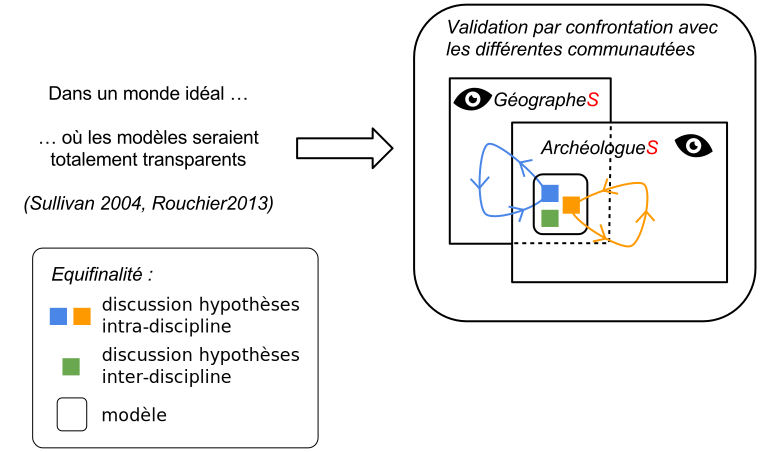
\includegraphics[width=0.9\linewidth]{vconfrontation.pdf}
  \end{sidecaption}
\end{figure}

Dans un \enquote{monde idéal}, où les modèles seraient totalement transparents (c'est-à-dire sans erreur, et dont la dynamique interne générale et propre à chaque hypothèse est complétement connue, voir figure \ref{fig:S_vconfrontation}) alors reste seulement en discussion les hypothèses, les implémentations d'hypothèses, et les critères d’évaluation choisis pour figurer au coeur du modèle. L’équifinalité impose donc qu’une partie de la validation (dont on sait qu’elle est contextuelle) s'opère dans cette confrontation avec les autres acteurs, et donc les autres points de vue de la communauté.

Ainsi plus que les solutions techniques qui restent avant tout des moyens, c'est dans le processus de discussion et d'échange autour des hypothèses et des critères admis dans les modèles que notre connaissance sur les phénomènes réels est aussi amenée à progresser. Cette confrontation n'est pas statique, elle mobilise aussi une relecture des raisonnements ayant porté l'intégration des hypothèses ou des critères au modèle. %Ce n'est qu'à ce prix que des discussions à même de susciter la modification, l'hybridation et donc l'amélioration de ces mêmes modèles peuvent être mis en oeuvre.

C'est exactement ce que nous dit \textcites{OSullivan2004,Millington2012}, il faut aller plus loin et donner toute ses chances à cette discussion, en exposant le raisonnement, et les discours développés avec et autour des modèles :

\foreignblockquote{english}[\cite{OSullivan2004}]{The process of model development, the possible outcomes it reveals and interpretations of those outcomes, taken together, constitute a geographical narrative, so that modellers become ‘makers’ of stories.}

Si l'on se place sur le plan de la reproductibilité, moins exigente et pourtant encore peu mise en oeuvre cette dernière décennie \autocite{Wilensky2007a}, l'objectif porté par O'Sullivan nous impose d'aller encore plus loin en permettant aussi la reproduction des raisonnements accompagnant la construction des modèles. La variabilité exposée lors de la construction du modèle, les différentes hypothèses, les différents critères, le jeu de leur mise en tension réciproque, tout cela devient partie intégrante d'une capsule temporelle autonome et reproductible qui peut être exportée, rejouée, modifiée, discutée auprès des autres modélisateurs \Anote{horizon_naif}. De ce fait cette confrontation avec la propriété d'équifinalité des systèmes complexes passe d'une explicitation souhaitée pour l'interdisciplinarité, à une explicitation plus que souhaitable, voire nécessaire pour la reconstruction et la discussion des raisonnements produits. Associé à la cumulativité et en donnant à voir autant ce qui marche, que ce qui ne marche pas dans nos modèles, on offre aussi cette possibilité d'une progression commune dans la déconstruction d'une partie de cette équifinalité. Comme le propose Denise Pumain, il s'agit de construire et de \enquote{défendre un projet unifié de quête d'intelligibilité} pour les sciences \autocite[157-158]{Mathieu2014}.

Seulement jusqu'à présent l'évaluation des modèles n'est pas censée avoir de sens une fois sortie de son contexte de création, il y a donc un effort évident à faire pour se doter de l'ensemble des moyens nécessaires à l'exposition de ce contexte. La notion de \enquote{laboratoire virtuel} traditionnellement limitée à l'expérimentation du modèle mute, se pare aujourd'hui d'une acception légèrement différente. Des chercheurs \autocites{Schmitt2014, Amblard2003} ont voulu étendre cette notion pour y inclure également l'ensemble des méthodes et outils jugés nécessaires à l'étude de ce premier niveau d'expérimentation que représente la construction d'un modèle de simulation (la variation des hypothèses dans le modèle), désignant par ce fait un niveau supplémentaire d’expérimentation (la variation des outils et méthodes pour construire et étudier le modèle). Il faut encore étendre et repenser l'analogie du \enquote{laboratoire virtuel}, faire de celui-ci une \enquote{place publique} et lui donner une profondeur temporelle afin de rejouer, en tout transparence, la construction des modèles au contact des données, des critères, des expérimentations \foreignquote{latin}{in vivo}.


\paragraph{Reintégrer la dimension temporelle}



 - construction des indicateurs devient aussi importantes
 - raisonnement se déroule dans un rapport concret à l'experimentation



\Anotecontent{hermann_hypothesis}{Le \textit{hypothesis-testing} proposé par Hermann propose d'évaluer avec ce critère la capacité du système simulé à reproduire dans sa dynamique des interactions constatés dans le système observé}

A ce titre la construction des indicateurs que l'on juge capable de caractériser correctement un système observé s'appuie sur une base de connaissance elle même résultat d'un construit. Ainsi, considérer comme pertinente la comparaison terme à terme d'une chaîne d'interaction entre système observés et système simulés \Anote{hermann_hypothesis} revient implicitement à accepter comme satisfaisante une longue et inévitable chaîne d'erreur cumulée, elle même issue d'un long processus de construction (les bases de données en science humaines ne se construisent pas en un jour) qui biaise tout autant la qualité des données initiales (construction d'enquête, de relevés, d'observations), que les structures qui les encadrent (un modèle de répartition par classe d'age par exemple). C'est pourtant sur cette base que le modélisateur doit s'appuyer pour extraire, au regard d'une expertise qui intègre un savoir aussi bien quantitatif que qualitatif, des hypothèses sur les composants et les interactions entre composants dont la pertinence de leur présence dans le modèle s'avère elle même discutable vis à vis de la question posé ..



En un sens, s'appuyer sur l'expression de dynamique \enquote{vraisemblables} pour formuler des hypothèses impactant la suite du raisonnement, et les mécanismes suivant à ajouter au modèle, tel que le propose en substance la \textit{face validity}, semble être une erreur pouvant couter beaucoup de temps de redéveloppement à posteriori.






L'abduction de part l'argument naturaliste évolutionniste qu'on lui prête,dépasse le simple cadre de la logique dans lequel de toute façon elle posait déjà problème, et n'intervient donc pas comme un moyen de preuve : \enquote{ On nous propose plutot d’envisager l’ensemble des démarches par lesquelles les chercheurs s’orientent vers les hypothèses qui semblent plausibles, en éliminant celles qui ne peuvent etre considérées comme pertinente. } A ce titre, \enquote{La démarche abductive permet un authentique gain de sens, une progression dans l’élucidation}


Un argument supplémentaire pour parler d'évaluation plutôt que de validation \autocite{Amblard2006}, car celle-ci s'inscrit dans un projet parallèle à l'activité de construction du modèle, dont la mise en œuvre implique sinon la construction au moins l'existence préalable d'hypothèses, et d'indicateurs pertinents sur le système observé; une expertise cumulé qui dépasse de loin en durée et en travail le seul projet de construction d'un modèle, et fait souvent intervenir un système de modèle dans une démarche de construction des connaissances de portée beaucoup plus large que cette seule construction de modèles de simulation. Un point que l'on a déjà abordé dans le paragraphe \ref{decorreler_validation} pour justifier d'une décorrélation des problématiques de la Validation vue sous l'angle réducteur de cette seule activité de modélisation multi-agents.


Que cela soit les paramètres, valeur de paramètres, hypothèses mobilisés, choix d'implémentation des hypothèses, critères d'évaluations ( fait stylisés ou données ) construit ou choisi, tout ces étapes ne peuvent être mis en oeuvre si on n'accepte pas de voir l'activité de modélisation pour la simulation comme parti prenante d'une activité de construction des connaissances plus globales. C'est ce qui rend aussi difficile l'évaluation de publication soutenant l'originalité d'un modèle de simulation par un public n'ayant pas connaissance de ce système de modèles et des interactions complexes et réflexives qui relient ceux ci, que cela soit en amont ou en parallèle de la construction des modèles de simulations.

Cette démarche globale a été plusieurs fois théorisé par les géographes \autocites{Besse2000, Sanders2000, Mathian2014}, et une application plus explicite des relations que peut entretenir un modèle de simulation avec d'autres type de modélisation (statistique, spatiales) peut être vu dans la thèse de Clémentine Cottineau \autocite{Cottineau2014a, Cottineau2014b}. 

De plus, il reste difficile donc d'éliminer une hypothèse présente dans le modèle en fonction de sa seule mise en défaut observés à un instant $t$ donné dans la construction d'un modèle, notamment lorsque la présence de celle ci fait sens du point de vue des objectifs qui ont été fixés par le modélisateur. 

D'autant plus qu'il faut aussi prendre en compte cette double dynamique dans lequel opère la construction et la complexification des modèles et des indicateurs pour en rendre compte. Une hypothèse valable à un instant $t$ ne le sera peut etre plus à un instant $t + 1$, ou inversement. 

Peut être n'était-ce simplement pas le moment pour intégrer cette hypothèse au modèle, celui-ci étant encore trop simple ? Peut être manquait-il des interactions pour que sa dynamique soit révélé ? Peut être que l'indicateur devant rendre compte de cette dynamique n'est pas adapté ? Peut être que l'implémentation proposé n'était tout simplement pas la plus adapté à ce moment là ? etc. 

Ce qui a mon sens soulève ici plusieurs remarques : 
- il est vraiment difficile de savoir ce qui va se passer avec l'intégration ou le retrait des hypothèses, ou des critères d'évaluation dans un modèle de simulation si on ne dispose pas d'un outil permettant d'évaluer systématiquement chacune de ces modifications, ce point est valable tout autant pour les approche KIDS que KISS.
- cette évaluation doit être mis en place de façon immédiate, dès que les premières questions sont posés à la structure causale du modèle, afin de ne pas biaisé le raisonnement construit par la prolongation d'une phase de \textit{face validity} pouvant très vite devenir problématique de part les redéveloppements qu'elle suppose dans le futur.
- malgré cela, il faut bien voire qu'une exploration des comportements du modèle, même complète, ne fera pas disparaitre ce problème, qui tient avant tout de l'avancement du raisonnement dans la construction du modèle.

Il reste donc à gérer cette possibilité de réengager les hypothèses et les critères à différents moments dans la construction des modèles, et soutenir une activité de construction cumulative qui ne soit pas \enquote{oublieuse} de cette autre espace temps dans lequel se construise les hypothèses et les différents critères mobilisés. 




Une des possibilités pour sortir de cette problématique est je pense double : 
- proposer un historique du raisonnement
- supporter l'équifinalité de façon explicite























------------- VRAC LUNDI







- Quelle connaissance cherche-t-on à confronter ?

	- multiplicité des critères ?
	T : équifinalité


Autre cadre ?

- Simulation comme modèle parmi les modèles
- L'activité de construction, seul motif pour justifier des hypothèses et des critères

 Une des premières questions auquelle on est tenté de répondre coincide avec la citation d'Amblard. Celui-ci nous indique un rapprochement avec des seuls faits stylisés, mais pourquoi ne pas directement comparer chacune des hypothèses mobilisés avec les critères quantitatif (données) dont on dispose ? 







La démonstration précédente nous indique plusieurs pistes de réflexions.

D'une part l'objectif de réalisation d'un modèle au réalisme uniquement structurel n'a pas de sens, même avec beaucoup d'hypothèses, car elle ne permet en aucun cas de garantir la justesse d'une comparaison entre données empiriques et simulés, et n'offre donc aucun critère d'arrêt pertinent dans l'activité de modélisation.





%Pourquoi ne pas envisager ici une validation externe basé sur une comparaison empirique et terme à terme des hypothèses constitutive entrant dans la structure causale du modèle ?

 


\paragraph{Reprendre le controle dans cette mise en tension}
\label{p:critere_evaluation}

%C'est ce rapprochement entre hypothèses et critères d'évaluation mobilisés qui est le véritable enjeu dans la construction des modèles explicatifs. %Ces critères peuvent être de deux types, quantitatif ou plus qualitatif comme les fait stylisés.


%\textcite{Hermann1967, Hermann1967b} propose d'établir non pas une méthode, mais une série de méthodes complémentaires, dont il détaille pour chacune d'elle les qualités et les faiblesses pour la comparaison entre système modélisé et système de référence. Chaque méthode constitue ce qu'il appelle un \textit{validation criteria}, un type de critère de validation générique dont le choix et la mise en œuvre effective est déterminé par le modélisateur en fonction des objectifs poursuivis.


% A deplacer et a remettre dans le flux au desssus ? 

%On retrouve une idée assez similaire mais peut être exposé de façon moins formalisée chez \textcite{Hermann1967} qui évoque bien aussi la nécessité d’une \enquote{validation multi-critères} interrogeant et renforçant par l'accumulation et la diversification de ces différents tests la crédibilité des composantes internes du modèle.


%Enfin il faut noter que les critères d'évaluation, au même titre que les hypothèses, ne sont pas forcément connus au moment ou l'implémentation du modèle démarre, dont il faut déjà justifier la construction

%Quel est la nature de ce rapprochement ? Enfin, comment peut-t-on \enquote{supporter au mieux} le modélisateur dans son nouveau role d'acteur de cette mise en tension ? 

% Penser à dire qu'il est toujours possible d'inférer sur la réalité, en établissant de nouvelles mesures, mais aussi de nouveaux modèles. C'est pour cela qu'il est important de considérer les modèles de simulation dans une chaine plus globale de construction des connaissances.   








%Il y a donc en permanence dans l'activité du modélisateur l'illustration de multiples tensions qui font de celle ci une expérience parmis d'autres, et nous rapproche déjà d'un point de vue plus proche d'une vision relativiste qu'objectiviste. L'historique d'un modèle se lisant tout autant au travers des choix d'hypothèses exercés par le modélisateur tout au long de son expérience de modélisation, que dans la lecture de l'objet finalisé. Une tension entre d'un coté la volonté d'expliquer des données par un ensemble d'hypothèses explicatives respectant un critère de parcimonie, et de l'autre coté cette volonté naturelle du modélisateur à tenter d'expliciter un maximum de cette variabilité vis à vis de la séries de données dont on dispose, et dont on sais par ailleurs que celle ci est déjà loin d'être neutre, exhaustive ou exempt d'erreurs.

=> Clementine avait une phrase bien pour ca ! (voir fiche)


Autrement dit la réponse aux questions posés au modèle de simulation, et donc par extension à nos connaissances incomplètes sur le fonctionnement supposé du réel dans la reproduction d'un phénomène donné, se trouve dans cette mise en tension volontaire entre hypothèses du modèle et critères d'évaluations mis en place pour en rendre compte.

Il semble que cette mise en tension se satisfait assez bien d'un cadre d'analyse basé sur l'activité de modélisation, ou les critères et les hypothèses ne sont pas tous nécessairement connu à l'avance, ni introduit de façon simultanée. Ce qui laisse la place au cours de cette confrontation à l'avénement d'une certaine surprise, à même de produire une connaissance, et de guider le choix des modélisateurs à chaque nouvelle étape dans la construction du modèle. 

% Les critères toutefois entretiennent un lien avec les hypothèses dont ils sont censé rendre compte, on peut donc imaginer que la parcimonie exprimé dans la construction des modèles puisse faire en lien des critères porteurs de cette connaissance exprimés sur le comportement du modèle. 

% Une remarque d'autant plus valable lorsque on sais que cette histoire se construit en confrontation avec la construction et la mise en oeuvre progressive des critères constitutif du système ciblé.

% Ce qui pose effectivement toujours la question de la nature des connaissances attendues dans une telle perspective.









% La question des modes de constructions
%Une solution élégante à été proposé par plusieurs auteurs, sous la forme d'une famille de modèle.


%, pas seulement en sociologie, mais également en géographie ou le spatial et le temporel donne encore un autre poids à cette grille de lecture. 

\paragraph{Montrer l'équifinalité dans l'évaluation des modèles}

Là ou ce cadre d'analyse propose de réaffirmer le statut explicatif des hypothèses insérés dans les modèles par un ancrage empirique plus important, une parcimonie, et surtout une épistémologie admettant l'existence possible d'une explication même si la chaine de causalité s'avère partielle ou lacunaire, nous avons suivi une toute autre trajectoire dans notre équipe.

Il a en effet été choisi de justifier cette équifinalité non pas en l'intégrant dans un nouveau cadre d'analyse, mais en la faisant plutôt apparaitre de façon explicite comme le résultat de nos démarches de raisonnement accompagnant la construction des modèles. Il ne s'agit plus de produire des modèles de simulation comme le résultat d'une histoire, qui resteront de toute façon toujours critiquable, et dont on ne verra jamais l'historique de construction, au profit de trajectoire dans des familles d'hypothèse constitutive des modèle qui intègre et donne justement à voir cette variabilité et ces aller retours possible dans les propositions.

Il y a je crois plusieurs avantages à voire dans cette solution, car elle permet d'intégrer la transformation des modèles dans le temps et dans les disciplines, tout en replacant la discussion comme un élément important dans la validation. Cet argument nous est donné par OSullivan 

\foreignblockquote{english}[\cite{OSullivan2004}]{It is clear that assessment of the accuracy of a model as a representation must rest on argument about how competing theories are represented in its workings, with calibration and fitting procedures acting as a check on reasoning. So, while we must surely question the adequacy of a model that is incapable of generating results resembling observational data, we can only make broad comparisons between competing models that each provide ‘reasonable’ fits to observations. Furthermore, critical argument and engagement with underlying theories about the processes represented in models is essential: no purely technical procedure can do better than this.}

Pour \autocite{OSullivan2004} cet argument est donc un leurre, car si ces procédures améliorent bien la connaissance du modèle, absolument aucune garantie ne peut être donnée sur la qualité et la transférabilité de cette connaissance pour l'étude de processus réel. Cela est d'autant plus vrai lorsqu'il s'agit de système complexes, dont la nature même empêche toute  mesure des dynamiques à l'oeuvre lors des processus d'émergence, et rend donc discutable toute comparaison possible avec des dynamiques simulées.

L'évaluation devient le moyen sans être la solution. La seule solution à l'équifinalité réside dans la confrontation des hypothèses intégré dans les modèles. 


Ainsi plus que les solutions techniques, c'est dans le processus de discussion et d'échange autour des hypothèses admises dans les modèles que notre connaissance sur les phénomènes réels est amenée à progresser. Par la mobilisation, l'hybridation, la confrontation de modèles ou briques de modèle issues d'angles de vues inter-disciplinaires,  on met en œuvre une grande discussion à même d'éclairer cette dynamique globale qui serait de toute façon insaisissable dans sa globalité. {cf transcidisciplinarité de morin ?}

\autocite{Rouchier2013} s'appuyant sur une définition de \todo{Gilbert et Artweiler} décrit cette forme de validation basée sur la réutilisation et l'enrichissement collectif des modèles comme étant post-moderne, \enquote{ dans la mesure ou elle base la valeur d'un modèle au regard de son usage par une communauté d'usagers }. Il y a donc dans le processus d'évaluation des modèles de simulation une dimension collective qui ne peut plus être niés dans l'établissement d'outil et de méthodologie . De façon plus générale, \autocite{Rouchier2013} évoque et décrit bien dans un article récent \enquote{  Construire la discipline \enquote{ Simulation Agent }} la nature de ce mouvement structurant qui œuvre dans la construction de communauté scientifique. Celui ci prend forme autour de revues revendiquant une large ouverture inter-disciplinaire, tel que JASSS, qui font alors office de catalyseur en supportant, relayant ces discussions de fond, à la fois sur le plan méthodologique et technique.

Pour pousser l'analogie du \enquote{laboratoire virtuel} encore plus loin, il s'agirait alors d'ouvrir ce laboratoire aux autres scientifiques, d'en faire \enquote{place publique} afin de montrer l'histoire de nos protocoles, de nos modèles, de nos résultats \foreignquote{latin}{in vivo}, en assumant au passage toutes les contraintes que cela suppose. Dès lors, comment ne pas mettre en relation la complexification de cette représentation avec une épistémologie des pratiques du laboratoire tel que développés par Ian Hacking, ou Bruno Latour , et d'évaluer nos experimentation au regard d'un réseau de résultat cohérent, et non plus de théories dont on ne peut pas plus donner au final de réalité qu'à celle donnés à nos expérimentation ?

Si les débats sur le plan de l'analogie entre expérimentation réelles et virtuelles sont encores brûlant, un certain nombre de différence et de points communs ont déjà été assurés, et permettent de manipuler cette analogie avec prudence. Et nombreux sont les chercheurs ayant déjà suivis une voie similaire, replacant l'abduction et ses différents supports dans la construction et l'évaluation des modèles, et en acceptant au préalable les préceptes d'Epstein, dans son fameux if you didn't grow it you didn't explain it ... %% A developper.

Il s'agit maintenant d'explorer cette épistémologie qui remet au premier plan la démarche exploratoire et les outils qui la supportent, semblable en plusieurs points aux

Faisant cela, l'autonomie du modèle se diffuse à l'autonomie des démarches, des outils qui la composent, et des personnes qui les manipulent.

Une trajectoire des modèles déjà constaté dans nos pratiques de modélisation \autocite{Banos2013}, l'inter-disciplinarité inhérentes aux systèmes complexes cautionnant ces migrations pour éclairer des objets complexes à l'aube de cette diversité de points de vues, par l'emploi de nouvelle théories, de nouvelles échelles de temps et d'espace, et impliquant la transformation, au delà du modèle, de la démarche accompagnante qui permet son évaluation.

Quelques auteurs progressent sur cette voie en sciences humaines et sociales, mais cela reste des cas relativement isolés \autocite{Ngo2012} \autocite{Schmitt2014} \autocite{Heppenstall2007} \autocite{Stonedahl2011a} entre autres.

Dans sa conclusion \autocite{Rouchier2013} mise sur le développement de la crédibilité de cette discipline dans les années à venir, grâce aux revues, aux règles de conduites édictées, et aux modèles repris et discutés au cœur de cette communauté \autocite{Hales2003}.



et Rouchier2013


Quelque chose que les sciences humaines et sociales savent faire.

Argumentation denise...


%%%%%%%%%%%%%%
Nécessaire de prendre en compte l'activité de construction :
- construction des hypothèque 
- construction des critères


L'activité de construction et de mobilisation des critères permettant de questionner le modèle lors de sa construction révèle en réalité une autre activité de modélisation, aussi questionnante et importante que la construction en elle-même du modèle de simulation. 

Replacer dans une dynamique de construction, les deux activités pourrait même apparaitre comme indissociable, la complexification des modèles apellant fort probablement l'introduction toujours plus grande de critères pour en mesurer la cohérence interne.

Or si il est courant d'établir un modèle conceptuel pour cristaliser un jeu d'hypothèse à mobiliser dans une simulation, la plannification des critères pour mesurer l'impact réel de ces hypothèses dans la dynamique du modèle est moins courante, et pourtant celle-ci semble tout autant nécessaire. Il faut dire aussi que ceux-ci, tout comme les mécanismes ajoutés, ne sont pas toujours connus par avance, et oblige là encore à voir l'activité de modélisation comme une activité de raisonnement qui mérite toute sa place dans les publications. L'histoire ayant mené à la construction d'un modèle et des critères qui l'acccompagne devenant aussi important et discutable que le résultat final publié.



Comme on l'a déjà discuté, la modélisation pour l'explication à besoin d'être confronté aux données si elle veut être prise au sérieux \autocite{Banos2013}.






Ces deux éléments permettent de relativiser cette problématique de l'équifinalité, qui n'est alors plus percu comme un problème sapant l'explication, mais comme une richesse d






De plus, il faut penser que le fait d'accepter qu'aucune causalité ne peux être avancé, c'est se condamner à la seule manipulation des corrélations statistiques, avec le risque de tomber dans un point de vue relativiste souvent clamé par l'approche herméneutique.






They look for an informative explanation, which incorporates additional understanding of the level of reality that the phenomena of study belong to. In our example, this means an explanation adding further understanding of social individuals.


































++ famille de modèles ++ va avec
++ famille de critères ++ 



%- Les problèmes identifiés comme des problèmes de données liés aux ABM dans les Anasazi par Grüne-Yanoff sont applicables en réalité à toutes les sciences humaines : l'absence, l'incomplétude, l'incertitude des données, et l'impossibilité de mesurer des phénomènes empecherai l'obtention d'une chaine de causalité complète, l'inférence abductive et la possibilité d'une explication concurrente renvoie automatiquement à une explication causale partielle, et rend la possibilité d'une chaine de causalité complète impossible.
%- les hypothèses en entrée n'ont jamais été falsifié pour approcher les données en sortie, comme le suppose Grüne-Yanoff.
 

tout comme d'ailleur cela n'avait pas convaincu ...  qui voyait dans cet multiplicité de combinaisons possible un aveux de faiblesse dans la capacité causale de ces modèles. 





L'équifinalité offre ce support pour confronter nos théories sur un objet social qu'il est impossible de tout façon impossible de voir dans son unicité.


Si on comprend les enjeux d'un tel projet, se pose alors les moyens de sa réalisation; la systématisation des évaluations avait déjà été annoncé comme un outil devant être mobilisé dès la pose des premières hypothèses, mais elle devient absolument nécessaire pour rendre cette fouille de modèles réaliste, et passé peut être à une échelle supérieure, celle de la construction et de l'étude de famille de modèles comme premier élément de réponse intégrateur de la pluralités des points de vues.

A ce titre, le recours au calibrage, et la recherche de cohérence interne dans les dynamiques pourraient passer pour une tentative de mieux définir par ce biais les processus en jeu dans un contexte réel. Pour \autocite{OSullivan2004} cet argument est encore un leurre, car toujours au vu de l'équifinalité, si ces procédures améliorent bien la connaissance du modèle, absolument aucune garantie ne peut être donnée sur l